% !TEX root = main.tex
% Подключение файла с настройками и подключенными пакетами
\documentclass[
candidate, % document type
subf, % use and configure subfig package for nested figure numbering
times new roman % use Times New Roman font as main
]{disser}

% Кодировка и язык
\usepackage[T2A]{fontenc} % поддержка кириллицы
\usepackage[utf8]{inputenc} % кодировка исходного текста
\usepackage[english,russian]{babel} % переключение языков
\usepackage{textgreek} % греческие букву в текстовом режиме

% Геометрия страницы и графика
\usepackage[a4paper, left=3cm, right=15mm, top=2cm, bottom=2cm]{geometry} % поля страницы
\usepackage{graphicx} % подключение графики
\usepackage{pdfpages} % вставка pdf-страниц

% Таблицы
\usepackage{array} % расширенные возможности для работы с таблицами
\usepackage{tabularx} % автоматический подбор ширины столбцов
\usepackage{dcolumn} % выравнивание чисел по разделителю

% Математика
\usepackage{bm} % полужирное начертание для математических символов
\usepackage{amsmath} % дополнительные математические возможности
\usepackage{amssymb} % дополнительные математические символы
\usepackage{algorithmic} % описание алгоритмов

% Библиография и ссылки
\usepackage{cite} % поддержка цитирования
%\usepackage[hidelinks]{hyperref} % создание гиперссылок
\let\oldref\ref
\renewcommand{\ref}[1]{(\oldref{#1})} % скобки вокруг ссылок

% Прочее
\usepackage{color} % работа с цветом
\usepackage{epstopdf} % конвертация eps в pdf
\usepackage{multirow} % объединение ячеек таблиц по вертикали
\usepackage{afterpage} % вставка материала после текущей страницы
\usepackage[font={normal}]{caption} % настройка подписей к рисункам и таблицам
\usepackage[singlespacing]{setspace} % один межстрочный интервал
\usepackage{fancyhdr} % установка колонтитулов
\usepackage{listings} % поддержка вставки исходного кода

% Установка шрифта Times New Roman
\usepackage{tempora}

% Создание нового типа столбца для выравнивания содержимого по центру
\newcommand{\PreserveBackslash}[1]{\let\temp=\\#1\let\\=\temp}
\newcolumntype{C}[1]{>{\PreserveBackslash\centering}p{#1}}

% Настройка стиля страницы
\pagestyle{fancy}      % Использование стиля "fancy" для оформления страниц
\fancyhf{}              % Очистка текущих значений колонтитулов
\fancyfoot[C]{\thepage} % Установка номера страницы в нижнем колонтитуле по центру
\renewcommand{\headrulewidth}{0pt} % Удаление разделительной линии в верхнем колонтитуле
\setlength{\parindent}{1.25cm} % Установка абзацного отступа

% Настройка подписей к изображениям и таблицам
\captionsetup{format=hang,labelsep=period}

% Установка глубины оглавления
\setcounter{tocdepth}{2}

% Указание папки для поиска изображений
\graphicspath{{images/}}

% Установка стилей страницы и главы
\pagestyle{footcenter}
\chapterpagestyle{footcenter}


%сдвиг в списк
\usepackage{enumitem}
\setlist{leftmargin=12.5mm}

%дополнительные математические операторы
\DeclareMathOperator{\diag}{diag}
\DeclareMathOperator{\Sqrt}{sqrt}
\DeclareMathOperator{\const}{const}
\DeclareMathOperator{\argmin}{argmin}
\DeclareMathOperator{\tr}{tr}
\newcommand{\intinf}{\int_{-\infty}^{+\infty}}
\DeclareMathOperator{\si}{Si}
\DeclareMathOperator{\cin}{Cin}

% метаданные PDF
%\hypersetup{
%	pdfauthor={Новиков А.А.},
%	pdftitle={Алгоритмы глубокого обучения для предсказания структуры белковых комплексов},
%	pdfkeywords={},
%	pdfsubject={},
%	pdfcreator={pdflatex},
%	pdflang={Russian}}

\begin{document}
	% Включение титульного листа
	%
\includepdf[pages={1-2}]{periphery/title_task.pdf}
	\begin{titlepage}
    \begin{center}
       \textbf{МИНИСТЕРСТВО ОБРАЗОВАНИЯ РЕСПУБЛИКИ БЕЛАРУСЬ}

       \textbf{БЕЛОРУССКИЙ ГОСУДАРСТВЕННЫЙ УНИВЕРСИТЕТ}

       \textbf{ФАКУЛЬТЕТ ПРИКЛАДНОЙ МАТЕМАТИКИ И ИНФОРМАТИКИ}

       \textbf{Кафедра математического моделирования и анализа данных}
    \end{center}

    \vspace{80pt}

    \begin{center}
        НОВИКОВ Антон Андреевич
    \end{center}

    \begin{center}
        \textbf{АЛГОРИТМЫ ГЛУБОКОГО ОБУЧЕНИЯ ДЛЯ ПРЕДСКАЗАНИЯ СТРУКТУРЫ БЕЛКОВЫХ КОМПЛЕКСОВ}
    \end{center}

    \begin{center}
        Магистерская диссертация

        специальность 7-06-0533-05
        <<Прикладная математика и информатика>>
    \end{center}

    \vspace{50pt}

    \hfill
    \begin{minipage}{0.5\linewidth}
        \begin{flushleft}
            Научный руководитель
    
            Тузиков Александр Васильевич
    
            доктор физико-математических наук, профессор
    
        \end{flushleft}
    \end{minipage}

    \vspace{110pt}

    Допущена к защите

    <<\underline{\hspace{20pt}}>> \underline{\hspace{100pt}} 2025 г.

    Зав. кафедрой математического

    моделирования и анализа данных

    Малюгин Владимир Ильич

    доктор экономических наук, кандидат

    физико-математических наук, профессор    

    \vspace{90pt}

    \begin{center}
        Минск, 2025
    \end{center}
\end{titlepage}
\setcounter{page}{2}
	
	% Содержание, Введение, Общая характеристика работы
	% RUSSIAN
\newpage
\addcontentsline{toc}{chapter}{ОБЩАЯ ХАРАКТЕРИСТИКА РАБОТЫ}

\begin{center}
	\textbf{\large ОБЩАЯ ХАРАКТЕРИСТИКА РАБОТЫ}
\end{center}


\textbf{Ключевые слова:} кейвордс dct ghbdt ndctgfd mfjgm jdfgm jmfg mjdjf gmjldfmjl gmdfl g
кейвордс dct ghbdt ndctgfd mfjgm jdfgm jmfg mjdjf gmjldfmjl gmdfl g
кейвордс dct ghbdt ndctgfd mfjgm jdfgm jmfg mjdjf gmjldfmjl gmdfl g
кейвордс dct ghbdt ndctgfd mfjgm jdfgm jmfg mjdjf gmjldfmjl gmdfl g
кейвордс dct ghbdt ndctgfd mfjgm jdfgm jmfg mjdjf gmjldfmjl gmdfl g


\textbf{Задачи исследования:}
\begin{enumerate}
	\item пункт 1
	\item пункт 2
\end{enumerate}


\textbf{Цель работы:} тут цель


\textbf{Объект исследования} является


\textbf{Предмет исследования} является


\textbf{Методы исследования:} методы методы


\textbf{Результаты работы}


\textbf{Области применения}


% BELARUSIAN
\newpage
\addcontentsline{toc}{chapter}{АГУЛЬНАЯ ХАРАКТЫРЫСТЫКА РАБОТЫ}
\begin{center}
	\textbf{\large АГУЛЬНАЯ ХАРАКТЫРЫСТЫКА РАБОТЫ}
\end{center}

\textbf{Ключавыя словы:} кейвордс dct ghbdt ndctgfd mfjgm jdfgm jmfg mjdjf gmjldfmjl gmdfl g
кейвордс dct ghbdt ndctgfd mfjgm jdfgm jmfg mjdjf gmjldfmjl gmdfl g
кейвордс dct ghbdt ndctgfd mfjgm jdfgm jmfg mjdjf gmjldfmjl gmdfl g
кейвордс dct ghbdt ndctgfd mfjgm jdfgm jmfg mjdjf gmjldfmjl gmdfl g
кейвордс dct ghbdt ndctgfd mfjgm jdfgm jmfg mjdjf gmjldfmjl gmdfl g

\textbf{Мэта работы:} тут цель

\textbf{Задачи исследования:}
\begin{enumerate}
	\item пункт 1
	\item пункт 2
\end{enumerate}

\textbf{Аб’ектам даследавання} является


\textbf{Метады даследавання} методы методы

\textbf{Вынікі работы}

\textbf{Вобласть ўжывання}


% ENGLISH
\newpage
\addcontentsline{toc}{chapter}{GENERAL DESCIPTION OF WORK}
\begin{center}
	\textbf{\large GENERAL DESCRIPTION OF WORK}
\end{center}

\textbf{Keywords:} кейвордс dct ghbdt ndctgfd mfjgm jdfgm jmfg mjdjf gmjldfmjl gmdfl g
кейвордс dct ghbdt ndctgfd mfjgm jdfgm jmfg mjdjf gmjldfmjl gmdfl g
кейвордс dct ghbdt ndctgfd mfjgm jdfgm jmfg mjdjf gmjldfmjl gmdfl g
кейвордс dct ghbdt ndctgfd mfjgm jdfgm jmfg mjdjf gmjldfmjl gmdfl g
кейвордс dct ghbdt ndctgfd mfjgm jdfgm jmfg mjdjf gmjldfmjl gmdfl g

\textbf{The object:} тут цель

\textbf{The objective:}
\begin{enumerate}
	\item item one
	\item item two
\end{enumerate}


\textbf{Research methods:} методы методы

\textbf{The results}

\textbf{Application}
	%\setcounter{page}{3}
\newpage
\renewcommand{\contentsname}{\centerline{\large ОГЛАВЛЕНИЕ}}
\tableofcontents

\newpage
\addcontentsline{toc}{chapter}{ВВЕДЕНИЕ}
%\onehalfspacing
\begin{center}
	\textbf{\large ВВЕДЕНИЕ}
\end{center}

Задача предсказания взаимодействия белков популярна среди биоинформатиков и специалистов в области структурной биологии уже на протяжении нескольких десятков лет. В последнее десятилетие, вместе с ростом актуальности нейронных сетей, были предложены новые подходы для решения этой задачи \cite{deep_methods}.

В предыдущих работах \cite{prip2023} было предложено новое представление для белковых молекул -- матрица косинусов. Данное представление использовалось в качестве входных и выходных данных полносвёрточной нейронной сети \cite{fully_conv}, предсказывавашей взаимодействие белок-белковой пары.
В рамках данной работы предпринята попытка далее развить данное представление, чтобы получить возможность применить формализм теории поля для описания белковых взаимодействий, после чего применить подходы глубокого машинного обучения, для нахождения соответствующих функций поля.
Таким образом, направление работы, в определённой степени, вернулось к классическому методу потенциалов.
	
	% Подключение глав (тут нумерация с 0)
	\newpage
\begin{center}
	\textbf{\large ГЛАВА 1}

	\textbf{\large ОПИСАНИЕ БЕЛКОВЫХ МОЛЕКУЛ И КОМПЛЕКСОВ И СВЯЗАННЫХ ЗАДАЧ}
\end{center}
\refstepcounter{chapter}
\addcontentsline{toc}{chapter}{1. ОПИСАНИЕ БЕЛКОВЫХ МОЛЕКУЛ И КОМПЛЕКСОВ И СВЯЗАННЫХ ЗАДАЧ}

%copypaste а там поглядим

Полипептиды – биополимерные органические соединения, являющиеся основой для всей, известной на данный момент, жизни. Они состоят из аминокислотных остатков, связанных пептидной связью. Полипептиды условно разделяют на пептиды (состоят из менее чем 50 остатков) и белки (более чем 50 остатков). Далее, будем говорить в основном о белках. Части аминокислотных молекул, участвующие в пептидной связи, образуют главную цепь белка. К главной цепи белка присоединены многочисленные боковые цепи – части аминокислотных остатков, не участвующие в пептидной связи, но определяющие функциональную роль соответствующих участков белка. Существует 20 основных аминокислот, встречающихся повсеместно. Кроме 20 основных, существуют другие, более редкие аминокислоты, однако на практике, ими всегда пренебрегают. При изучении белков, выделяют 4 уровня структуры:
\begin{enumerate}
\item Первичный уровень – это линейная последовательность аминокислотных остатков. Эта последовательность устанавливается с секвенированием. С одной стороны, этого уровня, самого по себе, не достаточно для решения большинства задач обработки белковых соединений. Однако, данный уровень кодирует все более высокие структурные уровни. Кроме того, первичный уровень позволяет устанавливать эволюционную близость между двумя белковыми соединениями.
\item Вторичный уровень – последовательные участки главной цепи белковой молекулы склонны образовывать регулярные структуры: β-листы, α-спирали; нерегулярные структуры: изгибы и петли; а также неупорядоченные участки (которые можно считать нерегулярной последовательностью очень коротких регулярных участков).
\item Третичный уровень – полная трёхмерная структура молекулы. Включает в себя структуры вторичного уровня, их взаимное расположение, а также положение всех боковых цепей. Представляет собой основной интерес, так как позволяет строить фармакофорную модель, проводить докинг с малыми молекулами, проводить анализ молекулярной динамики и т.д. Трёхмерную структуру полипептидной модели называют её свёрткой. 
\item Четвертичный уровень – существует для белковых молекул, образующих комплексы – соединения, образованные слабыми связями. Представляет собой третичные структуры всех компонент и их взаимное расположение. Часто встречаются комплексы, состоящие из нескольких одинаковых компонент. В зависимости от числа таких компонент, выделяют различные виды симметрий !!![1]. Важным отличием белков от пептидов в контексте четвертичного уровня является то, что большие белковые молекулы почти не изменяются структурно при взаимодействии друг с другом. В то же время пептид, при взаимодействии с большой белковой молекулой, может значительно поменять собственную свёртку.
Важными фундаментальными задачами являются предсказание сворачивания белка, предсказание взаимодействия белков и дизайн белков. Первая представляет собой предсказание третичной структуры по первичной; вторая – предсказание четвертичной структуры по третичной; третья – поиск первичной структуры, удовлетворяющей заданной третичной. Рассмотрим существующие методы и подходы к решению задачи предсказания взаимодействия.
\end{enumerate}
\section{Подходы к предсказанию взаимодействия}
Выделим несколько групп методов, используемых для предсказания взаимодействия. Первой такой группой будут методы свободного докинга. В них могут использоваться эмпирические поля, скоринговые функции (в том числе, полученные с помощью машинного обучения). Эти поля и функции соответствуют свободной энергии комплекса. Минимум энергии должен соответствовать искомой структуре. Таким образом решается многомерная (в случае взаимодействия двух неодинаковых молекул – 6-мерная) задача оптимизации !!![2]. В результате работы алгоритма получают множество потенциально корректных моделей, которое ранжируется. Оценивают эффективность алгоритма на основании того, как высоко окажется правильная модель в полученном рейтинге.

Второй группой являются методы, основанные на белковой ко-эволюции. Эти методы изначально разрабатывались для предсказания сворачивания белка  (это AlphaFold2 !!![3] и вдохновленные им алгоритмы !!![4]), однако оказались применимы и к задаче предсказания взаимодействия (AlphaFold-Multimer !!![5]). Данные методы, используют информацию о родственных белках (предоставленную в явном виде или выученную), чтобы построить третичную и четвертичную структуру. И хотя, в задаче предсказания свёртки, такие алгоритмы показывают точность, сравнимую с экспериментальными методами (рентгеноструктурный анализ, ЯМР-спектроскопия и т.д.), с задачей предсказания взаимодействия они успешно справляются примерно в половине случаев, что, в свою очередь, является лучшим результатом в области.

Третьей группой обозначим методы на основе шаблонов !!!![6]. В некотором смысле, такие алгоритмы являются классической версией алгоритмов второй группы. Этот подход так же применим к обеим задачам. Он основан на том наблюдении, что схожие участки в разных белках имеют тенденцию сворачивать/взаимодействовать сходно. Таким образом, имея базу известных свёрток/взаимодействий, поискав в ней фрагменты неизвестного соединения можно восстановить его структуру.

К последней группе отнесём различные методы глубокого обучения, предсказывающие интерфейс взаимодействия !!![7]. Их можно разделить на несколько категорий в зависимости от того, какие архитектуры сетей используются и как представлены входные данные.
\begin{itemize}
\item Методы, использующие в качестве входных данных первичную структуру, используют свёрточные и рекуррентные сети.
\item Методы, использующие представление, в которых используется трёхмерная структура, заданная через трёхмерные воксели, используют трёхмерные свёрточные нейронные сети.
\item Методы, использующие в качестве входных данных поверхности белковых молекул !!!![14], используют топологические свёрточные сети !!!![15].
\item Методы, использующие графовые представления белковых молекул, используют графовые нейронные сети.
\end{itemize}
В эту же категорию можно записать подход, при котором входными данными является представление структуры белка в виде двумерной карты расстояний !!!![8, 9]. При таком подходе используют полносвёрточные нейронные сети. Имея интерфейс взаимодействия, если необходимо, можно восстановить полную модель !!!![8].

Подход, описываемый в данной работе, является развитием как раз последнего подхода. Далее, отметим несколько методов оценки качества предсказаний.
\section{Оценка качества предсказаний}

Конвенциональным методом оценки качества предсказания является метрика RMSD (root mean squared deviation) – среднеквадратическое отклонение !!!![10], измеряемое в ангстремах. Обычно для расчёта этой метрики  используют лишь Cα-атомы главной цепи. Для димерных комплексов обычно фиксируют одну из компонент, и считают отклонение атомов второй (предсказанной) компоненты от их истинной позиции. Модель считают допустимой, если её RMSD меньше 10 ангстрем. Допустимые модели считаются тем качественнее, чем меньше их RMSD.

При оценке алгоритмов, предсказывающих интерфейс взаимодействия, полные модели зачастую не строят. Вместо этого оценивают сами карты интерфейсов. Предсказание этих карт, по сути, представляет собой задачу бинарной классификации, поэтому их оценивают метриками, применимыми в задачах бинарной классификации: точностью, полнотой, коэффициентом корреляции Мэтью !!!![7], площадью под кривой ROC (AUROC) !!!![11].

Существуют метрики оценки качества предсказаний, комбинирующие в себе два описанных выше метода. Такая метрика, например, используется в соревновании CAPRI !!!![12]. Такие метрики используются потому, что нередки ситуации, когда хорошо предсказанный интерфейс порождает плохую трёхмерную модель.










	\newpage
\begin{center}
	\textbf{\large 1. МАТРИЦЫ КОСИНУСОВ}
\end{center}
\refstepcounter{chapter}
\addcontentsline{toc}{chapter}{1. МАТРИЦЫ КОСИНУСОВ}

Матрицы косинусов как математический объект были предложены ранее в рамках курсовых и дипломной работ. Теоретические результаты предыдущих работ здесь будут изложены, по возможности, кратко и без доказательств, но систематично. Здесь они необходимы, прежде всего, для правильного изложения новых результатов, касающихся нового объекта -- релятивистской матрицы косинусов. Кроме того, терминология данной главы может местами отличаться от терминологии предыдущих работ, что связано с тем, что она ещё не устоялась, и требует некоторых изменений для большей систематичности.

\section{Базовые определения}
Пусть имеется некоторое гильбертово пространство $\mathcal{H}$ (в частном случае некоторое конечномерное евклидово пространство $\mathbb{R}^{k}$).
Пусть в данном пространстве задана последовательность точек (ломаная) $X = (\vec{x}_i)$, где $i = \overline{0,n}$. Обозначим $\vec{p}_{i} = \vec{x}_i - \vec{x}_{i-1}$, где $i = \overline{1,n}$, тогда \textit{ненормализованной матрицей косинусов} по ломаной $X$ будем называть квадратную матрицу вида:
\begin{equation}
	{C}_{E} = {(<\vec{p}_{i}, \vec{p}_{j}>)}_{ij} \in \mathbb{R}_{n,n}.
	\label{C_E_definition}
\end{equation}
Если выполняется условие:
\begin{equation}
	||\vec{p}_{i}|| = 1, i = \overline{1,n},
	\label{normalized_definition}
\end{equation}
то говорят о \textit{нормализованных матрицах косинусов} или собственно \textit{матрицах косинусов}. На практике, удобнее всего работать с нормализованными матрицами косинусов, ненормализованные матрицы косинусов могут возникнуть при некоторых операциях над обычными матрицами косинусов. Далее в работе, если не оговорено противное, будет подразумеваться наличие нормализации. 

Название матриц следует из того факта, что при условии \ref{normalized_definition}:
\begin{equation}
	{C}_{E} = {(<\vec{p}_{i}, \vec{p}_{j}>)}_{ij} = {(||\vec{p}_{i}|| ||\vec{p}_{j}|| \cos{\vec{p}_{i} \wedge \vec{p}_{j}})}_{ij} = {(\cos{\vec{p}_{i} \wedge \vec{p}_{j}})}_{ij}.
	\label{name_cosine}
\end{equation}
Объект, определенный выше, строится по и описывает одну ломаную. Пусть имеется две последовательности точек: $X' = (\vec{x'}_{i})$, где $i = \overline{0,m}$ и $X'' = (\vec{x''}_{j})$, где $j = \overline{0,n}$. Тогда аналогично \ref{C_E_definition} можно построить матрицу косинусов по двум ломаным $X'$ и $X''$:
\begin{equation}
	{C}_{X',X''} = {(<\vec{p'}_{i}, \vec{p''}_{j}>)}_{ij} \in \mathbb{R}_{m,n}.
	\label{C_X1X2_definition}
\end{equation}

Определения \ref{C_E_definition} и \ref{C_X1X2_definition} здесь фундаментальны, на практике полезны также матрица косинусов, кодирующая поворот ломаной $C_A$, и кодирующая вектор относительно ломаной ${C}_{\nu}$ -- они являются частными случаями \ref{C_X1X2_definition}. Здесь определим ${C}_{\nu}$, в следующей секции -- $C_A$:

Пусть задан некоторый вектор $\vec{\nu} \in \mathbb{R}^k$ и $X = (\vec{x}_{i})$ с $i = \overline{0,m}$, тогда \textit{матрицей косинусов задающей вектор} назовём матрицу вида:
\begin{equation}
	{C}_{\nu} = {(<\vec{p}_{i}, \vec{\nu}>)}_{ij} \in \mathbb{R}_{m,n},
	\label{C_nu_definition}
\end{equation}
здесь $n \ge 1$ не зависит от ни от $X$, ни от $\vec{\nu}$, а выбирается из других практических соображений.

Непрерывным обобщение матрицы косинусов можно назвать \textit{поверхностью косинусов}. Пусть $x(\alpha)$ - гладкая кривая $x : [0, l] \rightarrow \mathcal{H}$ и $\vec{p}(\alpha) = \frac{\partial{x(\alpha)}}{\partial{\alpha}}$. Тогда \ref{C_E_definition} можно переписать как:
\begin{equation}
	C({\alpha}_1, {\alpha}_2) = <\vec{p}(\alpha_1), \vec{p}(\alpha_2)>.
	\label{C_E_definition_cont}
\end{equation}
Таким образом, получаем действительную функцию о двух параметров $C : [0, l] \times [0, l] \rightarrow \mathbb{R}$.
Условие нормализации для \ref{C_E_definition_cont} выглядит следующим образом:
\begin{equation}
	||\vec{p}(\alpha)|| = 1, \forall{i} \in [0, l].
	\label{normalized_definition_cont}
\end{equation}
Использование непрерывной \ref{C_E_definition_cont} для вычислений затруденено. Гораздо удобнее исследовать и использовать матрицы.

\section{Свойства матриц косинусов}
Для исследования свойств описанных матриц, необходимо записать их в более удобном виде. Пусть речь идёт об евклидовом простанстве $\mathbb{R}^{k}$, тогда в нём можно ввести репер
$O = (\vec{x}_0, \vec{v}_1, ..., \vec{v}_k)$, пораждающий декартову систему координат. Тогда каждой точке $\vec{x}_i$ и вектору $\vec{p}_i$ можно поставить в соответствие координатный вектор-столбец $p_i \in \mathbb{R}_{k,1}$. Полученные столбцы координат $p_i$ можно объединить в матрицу $P = [p_1, ..., p_n] \in \mathbb{R}_{k,n}$. Тогда \ref{C_E_definition} и \ref{C_X1X2_definition} можно переписать как:
\begin{equation}
	C_E = P^\mathrm{T}P,
	\label{C_E_calc}
\end{equation}
\begin{equation}
	C_{X_1, X_2} = {P_1}^\mathrm{T}{P_2}.
	\label{C_X1X2_calc}
\end{equation}

Теперь, имея некоторую матрицу $A \in \mathbb{R}_{k, k}$ можно определить \textit{матрицу косинусов преобразования $A$}:
\begin{equation}
	C_A = P^\mathrm{T}AP.
	\label{C_A_calc}
\end{equation}

\subsection{Базовые свойства}
Приведём основные свойства матриц косинусов (без доказательств):
\begin{enumerate}
\item Все значения матриц косинусов лежат на отрезке $[-1, 1]$;
\item Все диагональные элементы матрицы $C_E$ равны $1$ (при отстутствии нормализации -- $||\vec{p}_i||$);
\item Матрицы косинусов не зависят от выбора декартовой системы координат;
\item Ранг матрицы $C_E$ равен размерности ломаной $X$;
\item Матрица $C_E$ - симметричная. Все её собственные значения неотрицательны, и в сумме равны $n$;
\item Ломаную $X$ (ломаные $X_1$ и $X_2$) можно восстановить из $C_E$ ($C_{X_1, X_2}$) с точностью до выбора системы координат, причём как для нормированных, так и для ненормированных матриц (в случае последних с $C_{X_1, X_2}$ необходимо знание длин векторов $\vec{p}_i$).
\end{enumerate}

\subsection{Восстановление исходных ломаных}
Последнее свойство наиболее важно, так как оно позволяет использовать матрицы косинусов как инвариантное представление геометричеких ломаных (что крайне полезно при исследовании белковых молекул и их взаимодействий). Зная \ref{C_E_calc} и \ref{C_X1X2_calc} легко построить соответсвующие матрицы. Ниже приведём без доказательств алгоритмы, которые позволяют строить ломаные по этим матрицам:

\begin{enumerate}
\item \textit{Восстановление $X$ из $C_E$}
Из описанного выше свойства 5 следует, что матрица $C_E$ будет обладать $k$ неотрицательными собственными значениями $\lambda_1, ..., \lambda_k$ и собственными векторами $v_1, ..., v_k \in \mathbb{R}_{n,1}$. Тогда в некоторой системе координат матрица $P$ примет вид:
\begin{equation}
	P = \diag(\sqrt{\lambda_1}, ..., \sqrt{\lambda_k}){[v_1, ..., v_k]}^\mathrm{T},
	\label{X_from_C_E_extraction}
\end{equation}
где координаты точек ломаной $X$ восстанавливаются из $P$ через кумулятивную сумму. Формула \ref{X_from_C_E_extraction} работает и для ненормализованных матриц.

\item \textit{Восстановление $X_2$ из $C_{X_1, X_2}$ при известном $X_1$}
Введём следующую крайне важную матрицу:
\begin{equation}
	T_P = {(P{P}^\mathrm{T})}^{-1}P,
	\label{T_definition}
\end{equation}
данная матрица (с поправкой на транспонирование) представляет собой матрицу вычисления параметров линейной регрессии. Из \ref{C_X1X2_calc} и \ref{T_definition} следует, что:
\begin{equation}
	T_{P_1}C_{X_1, X_2} = {(P_1{P_1}^\mathrm{T})}^{-1}P_1{P_1}^\mathrm{T}{P_2} = P_2,
	\label{X2_from_C_X1X2_extraction_known_X1}
\end{equation}
данная формула позволяет посчитать $P_2$ из $C_{X_1, X_2}$ при известном $P_1$, из которого, с помощью кумулятивной суммы, можно получить $X_2$. Формула \ref{X2_from_C_X1X2_extraction_known_X1}, опять же, работает и для ненормализованных матриц. Также с помощью такого подхожа можно восстановить вектор $\vec{\nu}$ из
\ref{C_nu_definition}.

\item \textit{Восстановление $A$ из $C_A$ при известном $X$}
Данная операция выполняется с помощью двойного применения матрицы \ref{T_definition}:
\begin{equation}
	T_PC_AT_P^\mathrm{T} = {(PP^\mathrm{T})}^{-1}P(P^\mathrm{T}AP)P^\mathrm{T}{(PP^\mathrm{T})}^{-1} = A,
	\label{A_from_C_A_extraction_known_X}
\end{equation}

\item \textit{Восстановление $X_1$ и $X_2$ из $C_{X_1, X_2}$}
Для выполнения данной операций существует следующий алгоритм, доказательство которого было приведено в предыдущей работе:
\begin{algorithmic}
\STATE 1.  Пусть $K_1$ -- матрица собственных векторов $C_{X_1,X_2}C^\mathrm{T}_{X_1,X_2}$;
\STATE 2.  Пусть ${K_2}$ -- матрица собственных векторов $C^\mathrm{T}_{X_1,X_2}C_{X_1,X_2}$;
\STATE 3.  $L_1 \gets K^\mathrm{T}_1C_{X_1,X_2}$;
\STATE 4.  $L_2 \gets (C_{X_1,X_2}K_2)^\mathrm{T}$;
\STATE 5.  $M \gets T_{L_2}C_{X_1,X_2}T^\mathrm{T}_{L_1}$;
\STATE 6.  Пусть $N$ -- матрица собственных значений $MM^\mathrm{T}$;
\STATE 7.  $O \gets N^\mathrm{T}ML_2$;
\STATE 8.  $s \gets T_{[O]^2}e$, где $e$ -- единичный вектор столбец;
\STATE 9.  $\hat{P}_1 = \diag(\Sqrt(s))O\diag(||\vec{p'}_1||, ..., ||\vec{p'}_m||)$;
\STATE 10. $\hat{P}_2 = T_{\hat{P}_1}C_{X_1,X_2}$.
\end{algorithmic}
\end{enumerate}

Описанные выше алгоритмы могут работать не только с истинными матрицами косинусов, но и с некоторыми приближёнными/зашумлёнными матрицами. Для этого достаточно производить нормализации по $||\vec{p}_i||$ там, где возникают матрицы $P$. В предыдущих работах было показана устойчивость описанных методов при добавлении случайных шумов.
 
\subsection{Арифметические свойства матриц косинусов}
\subsubsection{Сложение матриц $C_E$}
Пусть имеется две ломаные $X'$ в $\mathbb{R}^{k_1}$ и $X''$ в $\mathbb{R}^{k_2}$ имеющие соответствующие $P' = [p'_1, ..., p'_n] \in \mathbb{R}_{k_1,n}$ и $P'' = [p''_1, ..., p''_n] \in \mathbb{R}_{k_2, n}$.
Найдём сумму соответствующих им матриц $C'_E$ и $C''_E$:
\begin{equation}
	C'_E + C''_E = {P'}^\mathrm{T}P' + {P''}^\mathrm{T}P'' = {\begin{bmatrix} P' \\ P'' \end{bmatrix}}^\mathrm{T}{\begin{bmatrix} P' \\ P'' \end{bmatrix}} = {P^{+}}^\mathrm{T}P^{+} = C_E^{+},
	\label{C_E_sum}
\end{equation}
где получили новую ломанную $X^{+} = X' \oplus X''$ в $\mathbb{R}^{k_1 + k_2}$, а также $P^{+} = \begin{bmatrix} p'_1 & ... & p'_n \\ p''_1 & ... & p''_n \end{bmatrix} \in \mathbb{R}_{k_1 + k_2, n}$.
Таким образом сумма двух матриц косинусов -- ненормализованная матрица косинусов, которой соответствует ломаная, являющаяся прямой суммой ломаных-операнд.

\subsubsection{Вычитание матриц $C_E$}
Используя обозначения из \ref{C_E_sum} запишем:
\begin{equation}
	C'_E - C''_E = {P'}^\mathrm{T}P' - {P''}^\mathrm{T}P'' = {\begin{bmatrix} P' \\ iP'' \end{bmatrix}}^\mathrm{T}{\begin{bmatrix} P' \\ iP'' \end{bmatrix}} = {P^{-}}^\mathrm{T}P^{-} = C_E^{-}.
	\label{C_E_minus}
\end{equation}
Применяя разность в общем случае, придётся выйти из поля действительных чисел, и перейти к полю комплексных чисел. При том, что матрица $C_E^{-}$ всё еще действительная, порождающая её ломаная $X^{-} = X' \oplus iX''$ уже принадлежит $\mathbb{C}^{k_1 + k_2}$. Для матрицы, полученной из \ref{C_E_minus}, в общем случае не будет выполняться свойство о неотрицательности собственных значений. Из-за появления отрицательных собственных значений, при восстановлении $X^{-}$ из $C_E^{-}$ необходимо переписать \ref{X_from_C_E_extraction} как:
\begin{equation}
	P^{-} = \diag(\sqrt{\lambda_1^{+}}, ..., \sqrt{\lambda_{k_1}^{+}}, i\sqrt{-\lambda_1^{-}}, ..., i\sqrt{-\lambda_{k_2}^{-}}){[v_1^{+}, ..., v_{k_1}^{+}, v_1^{-}, ..., v_{k_2}^{-}]}^\mathrm{T}.
	\label{X_from_C_E_extraction_min}
\end{equation}

\subsubsection{Произведение матриц косинусов}
Раннее было показано, что произведение матриц косинусов может быть использовано для некоторых приближённых вычислений. Причины такого поведения, а также исследование
точности приближений здесь опустим, приведём лишь сами приближённые выражения.

Пусть $C_{X_1, X_2} \in \mathbb{R}_{m, n}$ и $C_{X_2, X_3} \in \mathbb{R}_{n, l}$, тогда:
\begin{equation}
	C_{X_1, X_2}C_{X_2, X_3} \approx \frac{n}{k}C_{X_1, X_3}.
	\label{mult_approx}
\end{equation}

Выражение \ref{mult_approx} приводит к следующим выражениям:
\begin{itemize}
\item $C_AC_B \approx \frac{n}{k}C_{AB}$;
\item Для ортогональных $A^\mathrm{T} = A^{-1}$ выполняется $C_A^\mathrm{T}C_A \approx C_AC_A^\mathrm{T} \approx \frac{n}{k}C_E$;
\item $C_EC_{X_1, X_2} \approx \frac{m}{k}C_{X_1, X_2}$;
\item $C_E^2 \approx \frac{n}{k}C_E$.
\end{itemize}

%\subsubsection{Применение свёрток к поверхностям косинусов}
%TO DO

%\subsection{Применение матриц косинусов}
%TO DO

\section{Релятивистская матрица косинусов}

В данном разделе представлен полностью новый результат, касающийся матриц косинусов. \textit{Релятивистская матрица косинусов $C_{rel}$} отличается от обычной $C_E$ тем, что позволяет закодировать не только лишь некоторую последовательность точек, но точку, из которой эта последовательность наблюдается. Таким образом получается инвариантное относительно выбора декартовой системы координат (а вообще говоря -- Лоренц-инвариантное) представление пары точка-ломаная, что позволяет задавать функции (поля), порождаемые ломаной (белковой молекулой), как преобразования матриц косинусов. Для релятивистских матриц будет дано полное определение, в соответствии со специальной теорией относительности (СТО), и приближённая запись, используемая на практике.

\subsection{Полное определение}

Пусть существует некоторая последовательность точек $X$, точки которой перемещаются в пространстве $\mathbb{R}^{k}$ со скоростями, не превышающими скорость света $c$:
\begin{align}
	X(t) = (\vec{x}_{l}(t)), l = \overline{0,n}; \\
	\vec{x}_l : \mathbb{R} \rightarrow \mathbb{R}^{k}; \notag \\
	||\frac{\partial{\vec{x}_l}}{\partial{t}}|| < c. \notag
\end{align}

Следуя Минковскому [ref!], в пространстве-времени можно ввести систему координат, в которой точке $\vec{x}_l$ в момент времени $t$ будет поставлен в соответствие вектор-столбец $x_l = [x^1_l(t), ..., x^k_l(t), ict]^\mathrm{T} \in \mathbb{C}_{k+1,1}$.

Пусть имеется некоторая точка $\vec{x}_{ref}$ и момент времени $t_{ref}$, из которых наблюдается ломаная $X$. Этой точке в пространстве-времени соответствуют координаты $x_{ref} = [x^1_{ref}(t), ..., x^k_{ref}(t), ict_{ref}]^\mathrm{T}$. Каждая точка из $X$ будет наблюдаться в $\vec{x}_{ref}$ в момент $t_{ref}$ при пересечении траектории $\vec{x}_l(t)$ и светового конуса, порождённого $\vec{x}_{ref}$ и $t_{ref}$. Из того, что все скорости не превышают $c$, следует, что такое пересечение единственно, и для каждой точки $\vec{x}_l$ произойдёт в некоторый момент времени $t^*_l \le t_{ref}$. Таким образом, в $\vec{x}_{ref}$ в момент $t_{ref}$ будет наблюдаться $X^*$ - образ ломаной $X(t)$ вида:
$X^* = (\vec{x}^*_l)$, где $l = \overline{0,n}$ и координаты $\vec{x}^*_l$ равны $x^*_l = [x^1_l(t^*_l), ..., x^k_l(t^*_l), ict^*_l]^\mathrm{T}$.

Если теперь посчитать $\vec{p}_l = \vec{x}^*_l - \vec{x}^*_{l-1}$ и использовать произведение Минковского, \ref{C_E_definition} или \ref{C_E_calc} можно получить \textit{релятивистскую матрицу косинусов}:
\begin{equation}
	C_{rel} = {(<\vec{p}_{l}, \vec{p}_{j}>)}_{lj} = {\left(\sum_{s=1}^{k} p^s_l p^s_j - c^2(t^*_l - t^*_{l-1})(t^*_j - t^*_{j-1})\right)}_{lj} \in \mathbb{R}_{n,n}.
	\label{C_rel_definition}
\end{equation}

Отметим, что требование нормализации \ref{normalized_definition} для релятивистских матриц косинусов будет иметь вид:
 \begin{equation}
	\sum_{s=1}^{k} {(p^s_l)}^2 = 1, l = \overline{1,n},
	\label{normalized_definition_rel}
\end{equation}
т.е. единичную длину должны быть только первые $k$ действительных компонент $p_l$ -- мнимая компонента $p^{k+1}_l$ может быть любой.

\subsection{Упрощённая формулировка}
Теперь, для упрощения, положим, что $\forall{l}: \vec{x}_l(t) = \vec{x}_l = \const$. Также, не нарушая общности, положим $t_{ref} = 0$. При таких предположениях вычисление пересечения светового конуса и траекторий заметно упростится, и можно будет записать:
\begin{equation}
	t^*_l = t_{ref} - \frac{||\vec{x}_l - \vec{x}_{ref}||}{c} = -\frac{1}{c}\sqrt{\sum_{s=1}^{k}(x^s_l - x^s_{ref})^2},
	\label{t_formula}
\end{equation}
и на основании \ref{t_formula} получим следующие значения координат:
\begin{equation}
	x^*_l = \begin{bmatrix} x^1_l \\ ... \\ x^k_l \\ -i\sqrt{\sum_{s=1}^{k}(x^s_l - x^s_{ref})^2} \end{bmatrix}.
	\label{x_formula}
\end{equation}

По \ref{x_formula} можно посчитать $P^* = \begin{bmatrix} P \\ -id \end{bmatrix} \in \mathbb{C}_{k+1,n}$ и по \ref{C_E_calc} посчитать:
\begin{equation}
	C_{rel} = {\begin{bmatrix} P \\ -id \end{bmatrix}}^\mathrm{T}\begin{bmatrix} P \\ -id \end{bmatrix} = P^\mathrm{T}P - d^\mathrm{T}d = C_E - d^\mathrm{T}d \in \mathbb{R}_{n,n}.
	\label{C_rel_definition_practical}
\end{equation}

В случае, когда $||\frac{\partial{\vec{x}_l}}{\partial{t}}|| \ll c$ разница между $\vec{x}_l(t^*_l)$ и $\vec{x}_l(t_{ref})$ будет иметь порядок вычислительной погрешности, а следовательно  использование \ref{C_rel_definition} неоправдано. Далее свойства матриц косинусов будем исследовать исключительно на основе \ref{C_rel_definition_practical}.

Можно видеть, что по аналогии с обычной $C_E$ можно получить матрицы аналогичные $C_{X_1, X_2}$, $C_A$, $C_\nu$:
\begin{equation}
	C_{rel, X_1, X_2} = {P^*_1}^\mathrm{T}{P^*_2} = {\begin{bmatrix} P_1 \\ -id_1 \end{bmatrix}}^\mathrm{T}\begin{bmatrix} P_2 \\ -id_2 \end{bmatrix} = C_{X_1, X_2} - d_1^\mathrm{T}d_2 \in \mathbb{R}_{m,n},
	\label{C_rel_X1X2_calc}
\end{equation}
\begin{equation}
	C_{rel, A} = {P^*_1}^\mathrm{T}A{P^*_2} \in \mathbb{C}_{n,n}.
	\label{C_rel_A_calc}
\end{equation}
Если матрица $A \in \mathbb{C}_{k+1,k+1}$ имеет структуру:
\begin{equation}
	A = \begin{bmatrix} A_{11} & iA_{12} \\ iA_{21} & -A_{22} \end{bmatrix},
	\label{good_A}
\end{equation}
где $A_{11} \in \mathbb{R}_{k,k}$, $A_{12} \in \mathbb{R}_{k,1}$, $A_{21} \in \mathbb{R}_{1,k}$, $A_{22} \in \mathbb{R}_{1,1}$; то для \ref{C_rel_A_calc} можно гарантировать:
\begin{align}
	C_{rel, A} &= {\begin{bmatrix} P \\ -id \end{bmatrix}}^\mathrm{T}\begin{bmatrix} A_{11} & iA_{12} \\ iA_{21} & -A_{22} \end{bmatrix}\begin{bmatrix} P \\ -id \end{bmatrix} = \notag \\
			    &= C_{A_{11}} + d^\mathrm{T}A_{12}P + P^\mathrm{T}A_{21}d + d^\mathrm{T}A_{22}d \in \mathbb{R}_{n,n}.
	\label{C_rel_A_calc_real}
\end{align}

Аналогично, можно построить $C_{rel, \nu}$ и гарантировать, что она будет действительной, если $\nu = [\nu_1, ..., \nu_k, i\nu_{k+1}]^\mathrm{T}$ ($\nu_l \in \mathbb{R}$).

Матрицы $C_{rel, A}$ и $C_{rel, \nu}$ позволяют кодировать матрицы и векторы в пространстве-времени, также как и $C_A$, $C_\nu$ кодировали матрицы и векторы в евклидовом пространстве.
Кроме того, аналогично \ref{C_E_definition_cont} можно ввести релятивистскую поверхность косинусов. Этот объект пригодится для доказательства одного из свойств $C_{rel}$.

\subsection{Свойства релятивистских матриц косинусов}
Свойства релятивистских матриц аналогичны свойствам обычных матриц:
\begin{enumerate}
\item Все значения $C_{rel}$ лежат на отрезке $[-2, 2]$;
\item Все диагональные элементы матрицы $C_{rel}$ лежат на отрезке $[0, 1]$;
\item Релятивистские матрицы косинусов не меняются от преобразований Лоренца (см. \ref{Lorenz_group});
\item Матрица $C_{rel}$ - симметричная. Одно её собственное значение отрицательно, остальные -- неотрицательны.
\end{enumerate}
Приведём доказательство первых двух свойств, а потом отметим особенности восстановления структур из описанных матриц.

Первое доказательство дадим для непрерывного случая. Пусть $\vec{x}(\alpha)$ - гладкая кривая $\vec{x} : [0, l] \rightarrow \mathbb{R}^k$,
и пусть, не нарушая общности, она наблюдается из $x_{ref} = [0, 0, 0, 0]^\mathrm{T}$. Тогда координаты вектора $\vec{x}(\alpha)$ будут иметь вид:
\begin{equation}
	x(\alpha) = \begin{bmatrix} x_{real}(\alpha) \\ -i||x_{real}(\alpha)|| \end{bmatrix} = \begin{bmatrix} x_1 \\ x_2 \\ x_3 \\ -i\sqrt{x_1^2 + x_2^2 + x_3^2} \end{bmatrix},
\end{equation}
и тогда:
\begin{equation}
	p(\alpha) = \frac{\partial x(\alpha)}{\partial \alpha} = \begin{bmatrix} \frac{\partial x_1}{\partial \alpha} \\ \frac{\partial x_2}{\partial \alpha} \\ \frac{\partial x_3}{\partial \alpha} \\
	-i\frac{x_1\frac{\partial x_1}{\partial \alpha} + x_2\frac{\partial x_2}{\partial \alpha} + x_3\frac{\partial x_3}{\partial \alpha}}{\sqrt{x_1^2 + x_2^2 + x_3^2}} \end{bmatrix} =
	\begin{bmatrix} \frac{\partial x_{real}(\alpha)}{\partial \alpha} \\ -i\cos\left(x_{real}(\alpha) \wedge \frac{\partial x_{real}(\alpha)}{\partial \alpha}\right) \end{bmatrix}.
\end{equation}
Условие нормализации \ref{normalized_definition_rel} тут имеет вид:
\begin{equation}
	||\frac{\partial x_{real}}{\partial \alpha}|| = 1.
	\label{normalized_definition_rel_cont}
\end{equation}
Теперь, аналогично \ref{C_E_definition_cont}:
\begin{align}
	C_{rel}(\alpha_1, \alpha_2) &= <p(\alpha_1), p(\alpha_2)> =
	\cos\left(\frac{\partial x_{real}(\alpha_1)}{\partial \alpha}\wedge\frac{\partial x_{real}(\alpha_2)}{\partial \alpha}\right) - \notag \\
	&- \cos\left(x_{real}(\alpha_1) \wedge \frac{\partial x_{real}(\alpha_1)}{\partial \alpha}\right)\cos\left(x_{real}(\alpha_2) \wedge \frac{\partial x_{real}(\alpha_2)}{\partial \alpha}\right).
	\label{C_rel_value_cont}
\end{align}
Из \ref{C_rel_value_cont} очевидно следует, что:
\begin{equation}
	\forall{\alpha_1, \alpha_2}: -2 \le C_{rel}(\alpha_1, \alpha_2) \le 2,
\end{equation}
а для случая $\alpha_1 = \alpha_2$:
\begin{equation}
	C_{rel}(\alpha, \alpha) = 1 - \cos^2\left(x_{real}(\alpha) \wedge \frac{\partial x_{real}(\alpha)}{\partial \alpha}\right) = \sin^2\left(x_{real}(\alpha) \wedge \frac{\partial x_{real}(\alpha)}{\partial \alpha}\right),
\end{equation}
\begin{equation}
	\forall{\alpha}: 0 \le C_{rel}(\alpha, \alpha) \le 1.
	\label{C_rel_value_cont_end}
\end{equation}

Формула \ref{C_rel_value_cont} крайне любопытна, так как она даёт альтернативную аналитическую форму записи поверхности косинусов, имеющую довольно понятное трактование.
Предложенное доказательство верно для гладкого случая, однако, если речь идёт о ломаной (и, соотвественно, матрице, а не поверхности), следует дать другое доказательство, которое, впрочем, также довольно тривиальное.

Пусть имеется $X = (\vec{x}_l)$, где $l = \overline{0,n}$, которая будет наблюдаться из точки $O$. Для $\forall{l} \in \{1, ..., n\}$ можно обозначить $A = \vec{x}_{l-1}$ и $B = \vec{x}_{l}$.
Пусть $\overline{OA} = d$ и $\overline{OB} = d + \Delta$. Предполагая нормализацию, будем также иметь $\overline{AB} = 1$. По известному свойству треугольников, будем иметь:
\begin{align}
	\overline{OB} \le \overline{OA} + \overline{AB}, \notag \\
	d + \Delta \le d + 1, \notag \\
	\Delta \le 1,
	\label{delta_le_1}
\end{align}
и
\begin{align}
	\overline{OA} \le \overline{OB} + \overline{AB}, \notag \\
	d \le d + \Delta + 1, \notag \\
	-1 \le \Delta.
	\label{min1_le_delta}
\end{align}
Из \ref{delta_le_1} и \ref{min1_le_delta} следует $|\Delta| \le 1$. Тогда $C_{rel}$ запишется как:
\begin{equation}
	C_{rel} = {\left({\begin{bmatrix} p^{real}_l \\ -i\Delta_l \end{bmatrix}}^\mathrm{T}\begin{bmatrix} p^{real}_j \\ -i\Delta_j \end{bmatrix}\right)}_{lj} = {({p^{real}_l}^\mathrm{T}p^{real}_j - \Delta_l\Delta_j)}_{lj},
\end{equation}
откуда аналогично \ref{C_rel_value_cont}-\ref{C_rel_value_cont_end} получаем первые 2 свойства.

\subsubsection{Восстановление исходных ломаных из релятивистских матриц}
Формула \ref{A_from_C_A_extraction_known_X}, а также \ref{X2_from_C_X1X2_extraction_known_X1} (для $C_{rel,\nu}$) применяются здесь так же, как и для обычных матриц косинусов.
В то же время применение \ref{X_from_C_E_extraction} затруднено, и хотя формула \ref{X_from_C_E_extraction_min}, казалось бы, здесь применима,
но наличие элемента $-i\sqrt{\sum_{s=1}^{k}(x^s_l - x^s_{ref})^2}$ в \ref{x_formula} приводит к тому,
что требуются некоторые дополнительные преобразования для согласования координат точек $\vec{x}_l$ и их расстояний до точки наблюдения.
Задача несколько упрощается, если известна структура ломаной, и необходимо восстановить только позицию точки наблюдения.

Хотя описанную выше задачу можно сформулировать и решать в терминах задачи оптимизации, эффективного алгоритма её решения пока не предложено.
Эксперименты показали, что её можно эффективно решать с помощью нейросетевых алгоритмов.
% TO DO расписать подробно





	\newpage
\begin{center}
	\textbf{\large 2. МОДЕЛЬ ВЗАИМОДЕЙСТВИЯ БЕЛКОВ}
\end{center}
\refstepcounter{chapter}
\addcontentsline{toc}{chapter}{2. МОДЕЛЬ ВЗАИМОДЕЙСТВИЯ БЕЛКОВ}
Цель данной главы -- предложить класс физических моделей, которые потенциально могут описывать взаимодействие белковых молекул.
В предыдущих работах [!ref] предлагалось напрямую предсказывать комформацию белковых комплексов с помощью полносвёрточных нейронных сетей,
и матрицы косинусов использовались в качестве инвариантной кодировки таких конформаций. В данной работе предлагается подход, близкий к классическому методу потенциалов.

\section{Лагранжев формализм классической релятивистской теории поля}
Опираясь на [!ref] кратко изложим суть данного формализма. Пусть имеется четырёхмерное пространство-время (трёхмерное пространство + время).
Пусть в данном пространстве можно задать $n$ обобщённых переменных:
\begin{equation}
	u_1(x_1, x_2, x_3, x_4), ..., u_n(x_1, ..., x_4);
	\label{generalized_variables}
\end{equation}
где $x_4 = ict$. У этих переменных можно вычислить
частные производные по каждой из координат: $\frac{\partial{u_1}}{\partial{x_1}}, ..., \frac{\partial{u_n}}{\partial{x_4}}$. Также могут использоваться производные
более высоких порядков, но в большинстве теорий обходятся лишь первым порядком.

Зададим действительнозначную $L(u_1, ..., u_n, \frac{\partial{u_1}}{\partial{x_1}}, ..., \frac{\partial{u_n}}{\partial{x_4}})$ -- \textit{функцию Лагранжа} или \textit{лагранжиан}.
В релятивистской теории на лагранжиан накладывается требование \textit{Лоренц-инвариантности}.

\textit{Преобразования Лоренца} -- это такие преобразования, которые сохраняют скалярные произведения в пространстве времени, т.е.:
\begin{equation}
	<f(x), f(y)> = <x, y>,
	\label{Lorenz_group}
\end{equation}
при условии, что для пространства-веремени скалярное произведение записывается как:
\begin{equation}
	<x, y> = x_1y_1 + x_2y_2 + x_3y_3 + x_4y_4 = x_1y_1 + x_2y_2 + x_3y_3 - c^2t_xt_y.
	\label{Minkowski_product}
\end{equation}

Из курса линейной алгебры известно, что преобразование $f$, обладающее свойством \ref{Lorenz_group}, является изометрическим, и ему буедт соответствовать
четырёхмерная комплексная ортогональная матрица $A$ ($A^\mathrm{T}=A^{-1}$) (не стоит путать с унитарной матрицей ($\overline{A}^\mathrm{T}=A^{-1}$)).

Если обобщённые координаты \ref{generalized_variables} задают скаляры, то их производные будут векторами, если переменные задают векторы, то их производные будут матрицами.
При Лоренц-преобразовании, заданном матрицей $A$ ($x \rightarrow Ax$), векторы и матрицы, входящие в лагранжиан, также будут изменяться
($v \rightarrow Av$; $M \rightarrow AMA^\mathrm{T}$). Требование Лоренц-инвариантности заключается в том, что преобразования Лоренца не должны изменять значение функции Лагранжа.

Если имеется Лоренц-инвариантный лагранжиан, то можно задать \textit{функцию действия}:
\begin{equation}
	S = \int_{spacetime}L(u_1, ..., u_n, \frac{\partial{u_1}}{\partial{x_1}}, ..., \frac{\partial{u_n}}{\partial{x_4}}) \, dx_1 \, dx_2 \, dx_3 \, dx_4.
	\label{action_function}
\end{equation}

Поведение системы, таким образом, описывается с помощью \textit{принципа стационарного действия}:
\begin{equation}
	S \rightarrow \min.
	\label{lagrangian_principle}
\end{equation}
Задачи типа \ref{lagrangian_principle} обычно решают с помощью вариационного исчисления. Из принципов вариационного исчисления и инвариантности относительно преобразований
\ref{Lorenz_group} следует теорема Нётер и автоматически выводимые из неё фундаментальные физические законы сохранения. Поэтому при моделировании белковых взаимодействий,
довольно привлекательно выглядит свойство Лоренц-инвариантности, так как с помощью него можно попытаться избежать явного учёта законов сохранения.

\section{Общая модель взаимодействия белков с применением релятивистских матриц косинусов}
Белковые молекулы являются полимерными молекулами. Они являются линейными последовательностями аминокислотных остатков, соединённых пептидными связями. В каждом из остатков
находится атом C\textalpha. В общем случае, знания пространственного расположения этих атомов и знания соответствующих аминокислтных остатков достаточно, чтобы полностью задать структуру белковой молекулы.
Кроме того, расстояние между соседними C\textalpha-атомами является практически константным, и равно 3,8\AA. Эти факты способствуют тому, чтобы можно было использовать матрицы косинусов для задания белковых структур.
Введение релятивистской матрицы косинусов \ref{C_rel_definition} позволяет задать как структуру молекулы, так и некоторую точку пространства-времени относительно неё. При этом, важным достоинством релятивистской матрицы является её Лоренц-инвариантность. Действительно, легко видеть, что от скалярных произведений, составляющих $C_{rel}$ в \ref{C_rel_definition}, в \ref{Lorenz_group} требуется инвариантность. Таким образом, если обычная матрица косинусов была инвариантна относительно изометрических преобразований в обычном евклидовом пространстве, то релятивистская матрица инвариантна относительно преобразований Лоренца в пространстве-времени. Следовательно, можно задавать обобщенные функции поля как функционалы над $C_{rel}$. Также необходимо отметить, что, так как $C_{rel}$ содержит в себе закодированным, в том числе, расстояние между точкой наблюдения и наблюдаемыми атомами, но делает это в неявной форме и без обращения этих расстояний, то при использовании описываемого подхода можно обойти проблему бесконечного роста функций поля при сближении атома и точки наблюдения.

Теперь дадим формальное описание данной модели в наиболее общем случае. Для начала, запишем:
\begin{equation}
	C_{rel} = C(X, \vec{x}_{ref}) \in \mathbb{R}_{m,m},
\end{equation}
где $X$ - последовательность точек -- C\textalpha-атомов описываемой молекулы в пространстве-времени, $\vec{x}_{ref}$ -- точка наблюдения, которой могут соответствовать координаты
$x_{ref} = [x_{ref}^1, x_{ref}^2, x_{ref}^3, x_{ref}^4] = [x_{ref}^1, x_{ref}^2, x_{ref}^3, ict_{ref}]$.
Тогда \ref{generalized_variables} можно выразить с помощью некоторого набора функционалов, принимающих на вход матрицу и данные об аминокислотной последовательности:
\begin{equation}
	u_l = F_l(C_{rel}, A) : \mathbb{R}_{m,m} \oplus \mathbb{A} \rightarrow \mathbb{C}; l=\overline{1..n}.
	\label{generalized_variables1}
\end{equation}

Тогда функция действия \ref{action_function} для одной белковой молекулы запишется как:
\begin{equation}
	S = \int_{spacetime}L(F_1(C(X, \begin{bmatrix} x_1 \\ x_2 \\ x_3 \\ x_4 \end{bmatrix}), A), ...,\frac{\partial{F_1(C(X, x), A)}}{\partial{x_1}}, ...) \, dx_1 \, dx_2 \, dx_3 \, dx_4.
	\label{action_function1}
\end{equation}

Если \ref{action_function} параметризовывалась обощенными функциями поля (т.е. решением \label{lagrangian_principle} были значения поля во всех точках пространства времени), то
\ref{action_function1} параметризуется ломаной $X(t)$ в пространстве-времени. Поэтому принцип стационарного действия \ref{lagrangian_principle} запишется как:
\begin{equation}
	X^{sol} = \argmin_{X}S.
	\label{lagrangian_principle1}
\end{equation}

Выражения \ref{action_function1} и \ref{lagrangian_principle1} описывают одну белковую молекулу, и, таким образом, задают модель её свёртки (без явного учёта растворителя и внешних сил).
Данные выражения легко обобщить на случай взаимодействия двух молекул, и далее на любое число белковых молекул, и даже на лиганды (для них, впрочем, в общем случае подход с релятивистской
матрицей косинусов и функционалом не подходит из-за нелинейности). Запишем модель для двух белковых молекул, описывамых парами $(X_1, A_1)$ и $(X_2, A_2)$:
\begin{equation}
	u_l(x) = F_l(C(X_1, x), A_1) + F_l(C(X_2, x), A_2), l=\overline{1..n};
	\label{generalized_variables2}
\end{equation}
\begin{align}
	S = \int_{spacetime}L(&F_1(C(X_1, x), A_1) + F_1(C(X_2, x), A_2), ...,\notag \\
						    &\frac{\partial{F_1(C(X_1, x), A_1)}}{\partial{x_1}} + \frac{\partial{F_1(C(X_2, x), A_2)}}{\partial{x_1}}, ... \notag \\
						    &) \, dx_1 \, dx_2 \, dx_3 \, dx_4;
	\label{action_function2}
\end{align}
\begin{equation}
	(X^{sol}_1, X^{sol}_2) = \argmin_{X_1, X_2}S.
	\label{lagrangian_principle2}
\end{equation}

Таким образом получили наиболее общую модель описания взаимодействия. При отстутствии явных выражений для \ref{generalized_variables1} аналитическое исследование такой системы невозможно. Впрочем, даже при наличии таких выражений, оно скорее всего было бы крайне сложным. Численный анализ и поиск таких функционалов также крайне затруднён, особенно с учётом того, что модель описывает полную динамику белковой молекулы, а экспериментальных данных такого рода де-факто не существует. Экспериментально получены лишь статические модели белковых молекул, а динамику получают с помощью рассчётов, полученных из теоретических соображений.

\section{Упрощённая модель взаимодействия белков}
Упростим предложенную модель по следующим пунктам:
\begin{enumerate}
\item Так как скорости движения белковых молекул крайне малы, по сравнению со скоростью света, то вместо полной релятивистской матрицы косинусов \ref{C_rel_definition} следует
использовать \ref{C_rel_definition_practical}.
\item Так как функционалы \ref{generalized_variables1} на практике будут аппроксимациями, полученными с помощью машинного обучения, то использование частных
производных от таких аппроксимаций может давать весьма сомнительные результаты (что связано с тем, что оператор дифференцирования не является непрерывным в теории функционального анализа), поэтому
опустим все явные вхождения частных производных в лагранжиан.
\item Так как вместе с этим опустится производная по времени, то, тем самым, будет получена статическая модель для белковых взаимодействий.
\item Для снижения количества степеней свободы, можно положить, как часто делают, что большие белковые молекулы жёсткие. Тогда они будут моделироваться как
абсолютно твёрдые тела, и будут параметризованы своим поворотом и сдвигом в пространстве.
\end{enumerate}
Применяя данные упрощения, мы более не будем иметь дело с релятивистской моделью, однако упрощённая модель всё еще может считаться некоторым
классическим механическим приближением такой общей модели.

Рассмотрим последствия предложенных упрощений:
\begin{align}
	X_1(t) = \const, \\
	X_2(t) = \const, \\
	X_1 = X_1(\alpha), \\
	X_2 = X_2(\alpha),
\end{align}
где $\alpha$ - обобщённый параметр, кодирующий взаимную конформацию молекул $X_1$ и $X_2$. Выражение \ref{generalized_variables1} остаётся без изменений.
Функция действия для одной молекулы примет вид:
\begin{align}
	S_1(\alpha) &= \int_{\mathbb{R}^3}L(F_1(C(X_1(\alpha), x), A_1), ...,F_n(C(X_1(\alpha), x), A_1)) \, dx_1 \, dx_2 \, dx_3 = \notag \\
				 &= \const,
	\label{action_function_single}
\end{align}
что обусловлено тем, что повороты и сдвиги не приведут к изменению суммарной функции действия. Функция действия двух молекул будет иметь вид:
\begin{align}
	S(\alpha) = \int_{\mathbb{R}^3}L(&F_1(C(X_1(\alpha), x), A_1)+F_1(C(X_2(\alpha), x), A_2), ..., \notag \\
                                                     &F_n(C(X_1(\alpha), x), A_1) + F_n(C(X_2(\alpha), x), A_2)) \, dx_1 \, dx_2 \, dx_3.
	\label{action_function_two}
\end{align}
Принцип стационарного действия примет вид:
\begin{equation}
	\alpha_{sol} = \argmin_{\alpha}S.
	\label{lagrangian_principle_practical}
\end{equation}

Из-за константности \ref{action_function_single} можно ввести \textit{частичный лагранжиан}:
\begin{align}
	L_{partial}(\alpha; x) &= L(F_1(C(X_1(\alpha), x), A_1)+F_1(C(X_2(\alpha), x), A_2), ...) - \notag \\
						   &- L(F_1(C(X_1(\alpha), x), A_1), ...) - L(F_1(C(X_2(\alpha), x), A_2), ...) = \notag \\
						   &= L(\alpha; x) - L_1(\alpha; x) - L_2(\alpha; x),
	\label{partial_lagrangian}
\end{align}
вычислив интеграл по которому, получим:
\begin{equation}
	\int_{\mathbb{R}^3}L_{partial}(\alpha; x) \, dx_1 \, dx_2 \, dx_3 = S(\alpha) - \const - \const,
\end{equation}
а следовательно:
\begin{equation}
	\alpha_{sol} = \argmin_{\alpha}\int_{\mathbb{R}^3}L_{partial}(\alpha; x) \, dx_1 \, dx_2 \, dx_3 = \argmin_{\alpha}S.
	\label{lagrangian_principle_practical_partial}
\end{equation}

Использование \ref{partial_lagrangian} будет полезно с численной точки зрения, а также весьма удобно при определённой степени линейности лагранжианов.

\section{Возможные варианты выбора функции Лагранжа}
\subsection{Скалярное поле}
В случае отсутствия частных производных, лагранжиан для скалярного поля $u$ примет вид:
\begin{equation}
	L(u) = au^2,
	\label{L_scalar}
\end{equation}
где $a$ - некоторая константа. Система ведёт себя принципиально разно при положительных и отрицательных $a$.

Модель с таким лагранжианом крайне бедна. Несколько обогатить её можно если использовать не одно, а $n$ скалярных полей:
$U = [u_1, ..., u_n]^\mathrm{T}$. Тогда имея некоторую постоянную $A \in \mathbb{R}_{n,n}$ запишем:
\begin{equation}
	L(U) = U^\mathrm{T}AU.
	\label{L_multiscalar}
\end{equation}
Таким образом получаем мультискалярное поле, функция Лагранжа которого -- квадратичная форма.
Мультискалярное поле отличается от векторного поля тем, что оно не меняется при преобразованиях Лоренца (ну или хотя бы при поворотах пространства).
Не нарушая общности, для квадратичных форм, можно считать $A$ -- симметричной ($A = A^\mathrm{T}$). Частичный лагранжиан будет иметь вид:
\begin{align}
	L_{partial}(U_1, U_2) &= L(U_1 + U_2) - L(U_1) - L(U_2) = \notag \\
						   &= (U_1+U_2)^\mathrm{T}A(U_1+U_2) - U_1^\mathrm{T}AU_1 - U_2^\mathrm{T}AU_2 = \notag \\
						   &=U_1^\mathrm{T}AU_2 + U_2^\mathrm{T}AU_1 = U_1^\mathrm{T}(A+A^\mathrm{T})U_2 = \notag \\
						   &=2U_1^\mathrm{T}AU_2.
	\label{L_partial_multiscalar}
\end{align}
Таким образом, частичный лагранжиан -- билинейная форма.

Матрица $A$ выражает взаимодействие различных полей друг с другом. Так как она симметричная, её можно диагонализировать (получим диагональную $A'$), и тем самым получить
набор новых полей $U' = [u'_1, ..., u'_n]^\mathrm{T}$, которые не будут взаимодействовать друг с другом, а только с самими собой. Вообще говоря,
абсолютные значения элементов $A'$ не важны, важны только их знаки, поэтому можно задать \ref{L_multiscalar} как:
\begin{equation}
	L(U') = {U'}^\mathrm{T}A'U'={\begin{bmatrix} U^+ \\ U^- \end{bmatrix}}^\mathrm{T}\begin{bmatrix} E & 0 \\ 0 & -E \end{bmatrix}\begin{bmatrix} U^+ \\ U^- \end{bmatrix},
	\label{L_multiscalar_diag}
\end{equation}
где лишние скалярные поля можно полагать нулевыми.

Функционал, способный задать скалярное поле, можно задать различными способами. Эксперименты показали, что наиболее практичный путь - следующий:
имея скаляр $u$, будем задавать вектор $v = [0, 0, 0, -iu]^\mathrm{T}$. Тогда \ref{generalized_variables1}, с помощью некоторого преобразования $G$, можно представить так:
\begin{equation}
	G : \mathbb{R}_{m,m} \oplus \mathbb{A} \rightarrow \mathbb{R}_{m,m},
\end{equation}
\begin{equation}
	C_{rel, v} = G(C_{rel}, A),
\end{equation}
\begin{equation}
	u = F(C_{rel}, A) = \begin{bmatrix} 0 & 0 & 0 &i \end{bmatrix}T_{X}G(C_{rel}, A)\begin{bmatrix} \frac{1}{m} \\ ... \\ \frac{1}{m} \end{bmatrix}.
	\label{scalar_F}
\end{equation}
Такое задание скалярное поля - это частный случай задания векторного поля, где собственно векторная часть нулевая.
При таком задании, повороты в пространстве не изменят поля, но преобразования Лоренца в общем случае могут вернуть векторную компоненту, что, впрочем, не
является большой проблемой, так как \ref{L_scalar} можно переписать как:
\begin{equation}
	L(v) = au^2 = a<v,v>.
	\label{L_scalar_vec}
\end{equation}

\subsection{Векторное поле}
Векторное поле задаётся вектором $v = [u_1, u_2, u_3, u_4]^\mathrm{T} = [v_1, v_2, v_3, iv_4]^\mathrm{T}$. Такое векторное поле не является чисто векторным, но также содержит в себе и скалярное.
Его лагранжиан можно задать с помощью \ref{L_scalar_vec} (легко видеть, что лагранжиан Лоренц-инвариантен) и аналогично \ref{L_multiscalar} обобщить на мультивекторный случай.
Формулу \ref{scalar_F} можно переписать так:
\begin{equation}
	v = F(C_{rel}, A) = T_{X}G(C_{rel}, A)\begin{bmatrix} \frac{1}{m} \\ ... \\ \frac{1}{m} \end{bmatrix}.
	\label{scalar_F}
\end{equation}

В общем и целом векторные поля, заданные таким образом, мало отличаются от скалярных. Главным отличием здесь является чувствительность к поворотам в пространстве,
что добавляет некоторых трудностей при обучении задаче предсказания взаимодействия белков. При этом модель оказывается не на много лучше мультискалярной модели.

% \subsection{Поле, заданное матрицей}
% Я думаю, для отчёта пока хватит и этого. 






	\newpage
\begin{center}
	\textbf{\large ГЛАВА 4}

	\textbf{\large ВСПОМОГАТЕЛЬНЫЙ МАТЕМАТИЧЕСКИЙ АППАРАТ}
\end{center}
\refstepcounter{chapter}
\addcontentsline{toc}{chapter}{4. ВСПОМОГАТЕЛЬНЫЙ МАТЕМАТИЧЕСКИЙ АППАРАТ}

В рамках данной главы описаны методы, которые применялись для компьютерной реализации теоретических моделей, изложенных в предыдущей главе.

\section{Конечномерная аппроксимация поля в пространстве}
Согласно \ref{generalized_variables}, для моделирования физической системы необходимо уметь задавать некоторые обобщённые переменные в пространсте-времени (пространстве). В данной работе основной формой такого задания являются нейронные сети (по схеме \ref{generalized_variables1}). Однако, для численного поиска минимума \ref{lagrangian_principle1} необходимо много раз производить  интегрирование, и каждое интегрирование требует своего определённого набора точек. В то же время, использование нейронной сети для вычисления в каждой такой точке может быть крайне трудоёмко, поэтому вполне логично, имея нейронную сеть и некоторую белковую молекулу, попробовать построить аппроксимацию поля, создаваемого данной молекулой, и задаваемого нейронной сетью. Использование подобной аппроксимации, хотя и само по себе трудоёмко, может в несколько раз ускорить процесс оптимизации \ref{lagrangian_principle1}. Далее описан подход, позволяющий с определённой долей успеха выполнить такую задачу. 

\subsection{Определение}
Для простоты начнём с одномерного случая. Пусть имеется непрерывная функция $f(x)$, $x \in \mathbb{R}$ такая, что $\exists \intinf f(x) \, dx \in \mathbb{R}$ и
$\lim_{x \to \pm\infty}f(x) = 0$. С помощью сигмоиды, переменной $x \in \mathbb{R}$ можно поставить в соответствие $t \in [0, 1]$:
\begin{equation}
	t = \frac{1}{1 + e^{-x}}.
	\label{t_and_x}
\end{equation}
Обратное преобразование выполняется с помощью функции логит:
\begin{equation}
	x = \ln\frac{t}{1-t}.
	\label{x_and_t}
\end{equation}
Зададим непрерывную функцию $g(t) = f(x) = f(\ln\frac{t}{1-t})$. Из свойств $f$ ясно, что:
\begin{equation}
	g(0) = g(1) = 0,
	\label{g_zeros}
\end{equation}
а также, что $\int_0^1g(t) \, dt \in \mathbb{R}$.

Из-за \ref{g_zeros} функция $g$ может быть продолжена как нечётная на $[-1, 1]$, а следовательно -- быть разложена в ряд Фурье по синусам:
\begin{equation}
	g(t) = \sum_{i=1}^\infty a_i\sin{\pi it},
	\label{fourier}
\end{equation}
где:
\begin{equation}
	a_i = 2\int_0^1g(t) \sin{\pi it} \, dt.
	\label{a_coef}
\end{equation}

Ряд \ref{fourier} сходится равномерно. Через него можно записать функцию $f(x)$:
\begin{equation}
	f(x) = \sum_{i=1}^\infty a_i\sin{\frac{\pi i}{1 + e^{-x}}},
	\label{logit_fourier}
\end{equation}
а коэффициент $a_i$ перепишется как:
\begin{equation}
	a_i = 2\int_0^1f(\ln\frac{t}{1-t}) \sin{\pi it} \, dt = 2\intinf f(x)\sin(\frac{\pi i}{1+e^{-x}})\frac{e^{-x}}{(1+e^{-x})^2}\, dx.
	\label{a_coef_logit}
\end{equation}
Раз \ref{fourier} сходится равномерно, то и \ref{logit_fourier} сходится равномерно.

Далее будет необходимо воспользоваться двумя известными функциями:
\begin{itemize}
\item $\si(x) = \int_0^x\frac{\sin t}{t}\, dt$ -- интегральный синус;
\item $\cin(x) = \int_0^x\frac{1 - \cos t}{t}\, dt$ -- интегральный косинус.
\end{itemize}

Если в \ref{fourier} имеем дело с разложением функции $g(t)$ по ортонормированному базису из функций $2\sin{\pi it}$, то в случае с \ref{logit_fourier}
последовательность функций $\sin{\frac{\pi i}{1 + e^{-x}}}$ не явлется ни нормированной, ни попарно ортогональной. Рассчитаем основные интегралы, связанные с \ref{logit_fourier}:
\begin{align}
	&\intinf\sin{\frac{\pi i}{1+e^{-x}}} \, dx = \int_0^1\sin{\pi it} \, d\ln{\frac{t}{1-t}} = \int_0^1 \frac{\sin{\pi it}}{t(1-t)} \, dt = \notag \\
	&= \int_0^1 \frac{\sin{\pi it}}{t} \, dt + \int_0^1 \frac{\sin{\pi it}}{1-t} \, dt = \int_0^1 \frac{\sin{\pi it}}{t} \, dt - \int_0^1 \frac{\sin{(\pi - \pi i\xi)}}{\xi} \, d\xi = \notag \\
	&= \int_0^1 \frac{\sin{\pi it}}{t} \, dt - {(-1)}^i\int_0^1 \frac{\sin{\pi i\xi}}{\xi} \, d\xi = (1 + {(-1)}^{i+1})\si(\pi i).
	\label{f_int}
\end{align}
Формула \ref{f_int} позволяет при наличии коэффициентов \ref{a_coef} посчитать интеграл функции $f(x)$ по всей числовой прямой. Пусть имеются две функции $f^1(x)$ и $f^2(x)$, которые разлагаются по \ref{logit_fourier} с коэффициентами $a^1_i$ и $a^2_j$. Крайне полезно уметь считать интеграл $\intinf f^1(x)f^2(x)\, dx$ (сравните с \ref{action_function_two} и \ref{L_partial_multiscalar}), что было бы крайне легко, если бы последовательность функций $\sin{\frac{\pi i}{1 + e^{-x}}}$ была ортонормированной, но так как это не так, необходимо рассчитать интегралы попарных произведений функций этой последовательности:

\begin{align}
	&\intinf\sin{\frac{\pi i}{1+e^{-x}}}\sin{\frac{\pi j}{1+e^{-x}}} \, dx = \int_0^1\sin{\pi it}\sin{\pi jt} \, d\ln{\frac{t}{1-t}} = \notag \\
	&= \int_0^1\frac{\cos\pi (i-j)t - \cos\pi (i+j)t}{2}\left(\frac{1}{t} + \frac{1}{1-t}\right)\, dt = \frac{1}{2}(\int_0^1\frac{1-\cos\pi (i+j)t}{t}\, dt - \notag \\
	&- \int_0^1\frac{1-\cos\pi (i-j)t}{t}\, dt + \int_0^1\frac{\cos\pi (i-j)t-\cos\pi (i+j)t}{1-t}\, dt) = \frac{1}{2}(\cin(\pi(i+j)) -\notag \\
	&- \cin(\pi(i-j)) + \int_0^1\frac{{(-1)^{i-j}}\cos\pi(i-j)\xi - {(-1)^{i+j}}\cos\pi(i+j)\xi}{\xi}\, d\xi) = \notag \\
	&= \frac{1+{(-1)}^{i+j}}{2}\left(\cin(\pi(i+j)) - \cin(\pi(i-j))\right).
	\label{fg_int}
\end{align}

Из \ref{fg_int} при $i=j$ получим:
\begin{equation}
	\intinf\sin^2\frac{\pi i}{1+e^{-x}}\, dx = \cin(2\pi i).
	\label{f_sqr_int}
\end{equation}

Так как в рамках исследуемой задачи необходимо аппроксимировать функции заданные на трёхмерном, а не одномерном пространстве, то следует перейти к трёхмерному ряду Фурье.
Для такого ряда формулу \ref{logit_fourier} перепишем как:
\begin{equation}
	f(x,y,z) = \sum_{i,j,k=1}^\infty A_{i,j,k}\sin{\frac{\pi i}{1 + e^{-x}}}\sin{\frac{\pi j}{1 + e^{-y}}}\sin{\frac{\pi k}{1 + e^{-z}}},
	\label{logit_fourier_3d}
\end{equation}
где:
\begin{equation}
	A_{i,j,k} = 2^3\iiint_{\mathbb{R}^3}\frac{f(x, y, z)\sin\frac{\pi i}{(1+e^{-x})^2}\sin\frac{\pi j}{(1+e^{-y})^2}\sin\frac{\pi k}{(1+e^{-z})^2}e^{-x-y-z}}{(1+e^{-x})^2(1+e^{-y})^2(1+e^{-z})^2}\, d^3x.
	\label{a_coef_logit_3d}
\end{equation}

Легко видеть, что формулы \ref{f_int}, \ref{fg_int} и \ref{f_sqr_int} полезны и для трёхмерного случая.

\subsection{Вычисление коэффициентов по методу Монте-Карло}

При построении аппроксимации, во-первых, приходится ограничиваться некоторым конечным числом слагаемых ряда, а во-вторых, необходимо численно получать значения коэффициентов \ref{a_coef_logit_3d}. Из-за относительно большой размерности функции, и необходимости считать интегралы по всему пространству, интегрирование по сетке точек не так удобно -- проще применить метод Монте-Карло.

Для метода Монте-Карло необходимо иметь некоторую трёхмерную случайную величину $\xi = {[\xi_x, \xi_y, \xi_z]}^\mathrm{T}$, принимающую все значения из $\mathbb{R}^3$ с распределением вероятности $p(x, y, z)$ ($p > 0$, $\iiint_{\mathbb{R}^3}p(x, y, z)\, dx\, dy\, dz = 1$). На роль такой случайной величины хорошо подходит многомерное нормальное распределение. Хорошо известно, что для любой функции $f(x, y, z)$ можно записать:
\begin{equation}
	\iiint_{\mathbb{R}^3}f(x,y,z)\, dx\, dy\, dz=\iiint_{\mathbb{R}^3}\frac{f(x,y,z)}{p(x,y,z)}p(x,y,z)\, dx\, dy\, dz=\E{\frac{f(\xi)}{p(\xi)}},
	\label{monte-carlo1}
\end{equation}
из чего, при наличии $N$ выборочных значений $\xi^i$, через статистическую оценку среднего получаем:
\begin{equation}
	\iiint_{\mathbb{R}^3}f(x,y,z)\, dx\, dy\, dz=\E{\frac{f(\xi)}{p(\xi)}} \approx \frac{1}{N}\sum_{i=1}^N\frac{f(\xi^i)}{p(\xi^i)}.
	\label{monte-carlo2}
\end{equation}
Использование формулы \ref{monte-carlo2} совместно с \ref{a_coef_logit_3d} даёт искомую аппроксимацию.

Достоинством описанного выше метода является, как минимум, то, что он работает, и позволяет с некоторой точностью записать многомерную, заданную на всём бесконечном множестве функцию, используя конечное число параметров. Следует также привести недостатки данного метода:
\begin{enumerate}
\item При ограниченном числе членов ряда, точность приближения крайне чувствительна к сдвигам приближаемой функции ($f(x, y, z) \to f(x+c_x, y+c_y, z+c_z)$). Это выражается в том плане, что  не следует сразу использовать \ref{a_coef_logit_3d}, вместо этого следует искать такое преобразование исходных координат -- желательно линейное $x = A\hat{x} + b$, для которого отклонение аппроксимации $\hat{f}$ от исходной $f$ будет минимальным:
\begin{align}
	&A'_{i,j,k} = 2^3\iiint_{\mathbb{R}^3}\frac{f(Ax+b)\sin\frac{\pi i}{(1+e^{-(a_{11}x+a_{12}y+a_{13}z+b_1)})^2}\cdot...\cdot e^{-((a_{11}+...)x+...)}}{(1+e^{-(a_{11}x+a_{12}y+a_{13}z+b_1)})^2\cdot...}\, d^3x,
	\label{a_coef_logit_3d_mod}
\end{align}
\begin{equation}
	\hat{f}(x,y,z) = \det(A)\sum_{i,j,k=1}^\infty A'_{i,j,k}\sin{\frac{\pi i}{1 + e^{-(a_{11}x+a_{12}y+a_{13}z+b_1)}}}\cdot...,
	\label{logit_fourier_3d_mod}
\end{equation}
и
\begin{equation}
	\iiint_{\mathbb{R}^3}{(f(x) - \hat{f}(x))}^2\,d^3x \to \min.
	\label{a_coef_logit_3d_mod_cond}
\end{equation}
Поиск \ref{a_coef_logit_3d_mod_cond} эффективно выполняется с помощью методов градиентного спуска.

\item Точность приближения также сильно зависит от дисперсии распределения $\xi$. Если дисперсия слишком мала, она может не покрыть всех особенностей функции $f$.

\item Увеличение количества учитываемых членов ряда Фурье приводит к увеличению точности, но в многомерном случае приводит к очень быстрому росту трудоёмкости вычислений, а формулы \ref{f_int}, \ref{fg_int} и \ref{f_sqr_int} становятся малоприменимыми.

\item Метод Монте-Карло обладает высокой дисперсией, его точность растёт со скоростью $O(\frac{1}{\sqrt{N}})$. Вместе с разложением в ряд Фурье и недостаточно большими значениями $N$ приводят к быстрому накоплению ошибок.
\end{enumerate}

\subsection{Графические примеры}
Приведём несколько графических примеров описанного выше подхода для аппроксимации одномерных функций и двумерных изображений.
\begin{figure}[H]
	\centering
	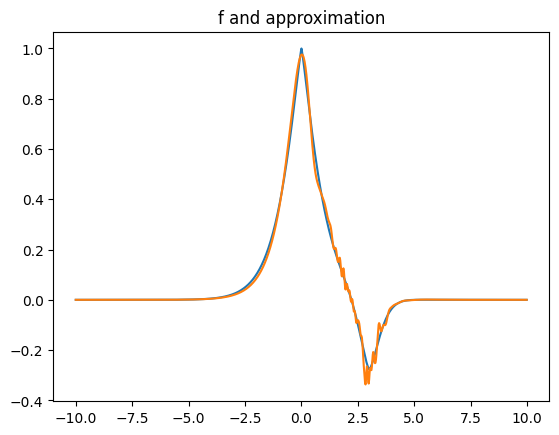
\includegraphics[scale=0.9]{plot1.png}
	\caption{Приближение функции $f(x) = e^{-|x|^{1,2}} - 0,3e^{-2|x-3|^{1,5}}$.}
	\label{fig_plot1}
\end{figure}
\begin{figure}[H]
	\centering
	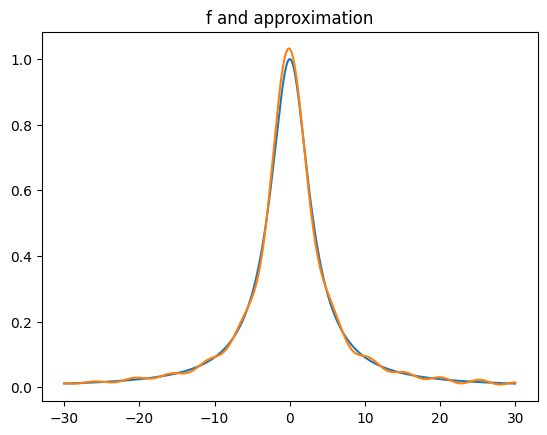
\includegraphics[scale=0.9]{plot2.png}
	\caption{Приближение функции $f(x) = \frac{10}{10 + x^2}$.}
	\label{fig_plot2}
\end{figure}
\begin{figure}[H]
	\centering
	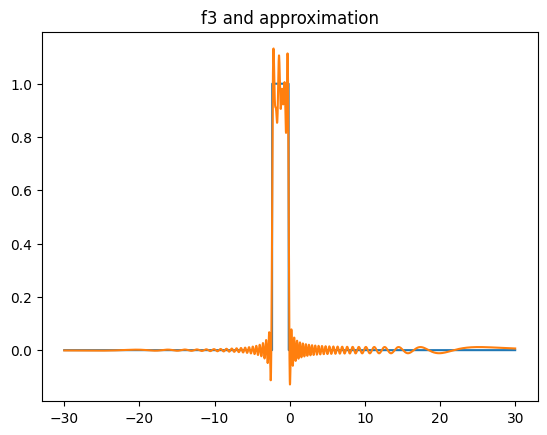
\includegraphics[scale=0.9]{plot3.png}
	\caption{Приближение функции $f(x) = \mathbb{I}[|x + 1,25| < 1,1]$.}
	\label{fig_plot3}
\end{figure}
\begin{figure}[H]
	\centering
	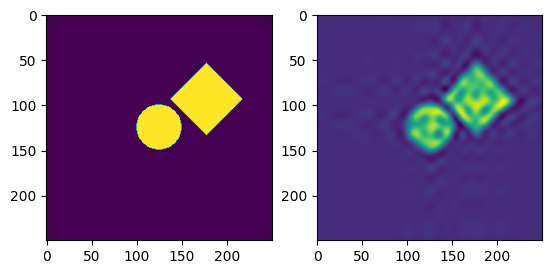
\includegraphics[scale=0.8]{imag1.png}
	\caption{Приближение круга и квадрата.}
	\label{fig_imag1}
\end{figure}
\begin{figure}[H]
	\centering
	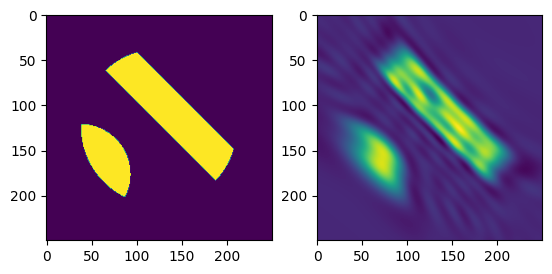
\includegraphics[scale=0.8]{imag2.png}
	\caption{Приближение пересечения круга с объединением круга и прямоугольника.}
	\label{fig_imag2}
\end{figure}
\begin{figure}[H]
	\centering
	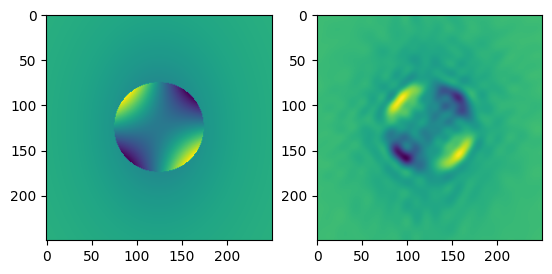
\includegraphics[scale=0.8]{imag3.png}
	\caption{Приближение функции $f(x, y) = \frac{xy}{10}\mathbb{I}[|x^2 + y^2| < 4] - \frac{1}{10 + x^2 + y^2}$.}
	\label{fig_imag3}
\end{figure}

\section{Параметризация пары взаимодействующих молекул}
Взаимодействие двух белковых молекул проще всего моделировать как взаимодействие двух жёстких тел. В общем случае, все конформации получаемого комплекса можно записать с помощью 6 параметров: одна компонента фиксируется, для второй компоненты выбирается центр (3 параметра) и поворот (3 параметра). В случае, когда компоненты идентичны (гомодимерные комплексы), в силу определённой симметрии, можно обойтись всего 4 параметрами.

Воспользовавшись физическими соображениями, можно попробовать сократить необходимое число параметров на 1. Для этого можно воспользоваться \textit{операцией <<сталкивания>>}\cite{prip2023}. Она заключается в том, чтобы найти такое минимальное расстояние между молекулами, при котором минимальное расстояние между C\textalpha-атомами не превышает некоторой границы (обычно ван-дер-ваальсовых радиусов атомов углерода -- 3,4\AA{}, но можно, например, 3,6\AA{}). Ранее, такая операция выполнялась с помощью итеративного процесса, при котором молекулы раздвигаются с некоторым постоянным шагом, пока условие о ненарушении границ не будет выполнено. В рамках же данной работы операция выполняется с помощью метода дихотомии.

При использовании моделей типа \ref{action_function}, необходимо выполнение интегрирования по всему пространству, что может быть выполнено с помощью метода Монте-Карло \ref{monte-carlo2}. Поиск решения \ref{lagrangian_principle_practical} заключается в итеративном интегрировании \ref{monte-carlo2}, изменении параметров комплекса, дальнейшем интегрировании, изменении параметров и т.д. Если при каждом интегрировании \ref{monte-carlo2} случайная выборка $\xi^i$, $i=\overline{1,N}$ генерируется заново, то возникает дополнительная дисперсия, которая мешает процессу оптимизации. Чтобы избежать этой проблемы, можно сгенерировать единое случайное облако $\xi^i$, $i=\overline{1,N}$ и применять его на всех итерациях. Впрочем, возникает проблема такого рода, что такое фиксированное облако может оказаться слишком маленьким и не покрывать всех возможных конформаций комплекса.

Чтобы как-то обойти данную проблему, можно использовать другую параметризацию. В ней центры молекул задаются через параметр $r$ как: $[-r, 0, 0]^\mathrm{T}$ и $[r, 0, 0]^\mathrm{T}$. Поворот каждой из молекул задаётся 3 параметрами, что приводит к тому, что итоговое количество параметров равно 7 (если использовать операцию сталкивания для поиска параметра $r$ при заданных поворотах, то можно сократить количество параметров до 6). Тогда случайную величину $\xi$ можно генерировать из многомерного нормального распределения, достаточно протяжённого относительно оси $[1, 0, 0]^\mathrm{T}$.

\section{Алгоритмы оптимизации}
В рамках данного исследования были использованы различные методы оптимизации. При обучении нейронный сетей, а также при решении \ref{a_coef_logit_3d_mod_cond}, используется популярный алгорит стохастической оптимизации Adam\cite{adam}. Впрочем, при решении \ref{lagrangian_principle_practical} данный алгоритм оказался малоприменим. Во-первых, при моделировании часто использовались плохо дифференцируемые функции. Во-вторых, из-за наличия малой относительно малого (по сравнению с нейронными сетями) количества параметров, алгоритм не способен достичь глобального минимума. Для решения данных проблем, предлагается использовать эволюционные методы оптимизации \cite{evol_methods}.

\subsection{Простой эволюционный алгоритм}
Был использован простой эволюционный алгоритм следующего вида. Пусть $p$ -- вектор параметров (кодирует форму взаимодействие), $f(p)$ -- минимизируемая функция (частичный лагранжиан),
$g(p)$ -- бинарная функция, сигнализирующая некорректные параметры (функция, сигнализирующая нарушение радиусов ван-дер-ваальса):
\begin{algorithm}
\begin{algorithmic}
\State $P \gets [p_1, p_2, ..., p_N]$ из многомерного равномерного распределения с заданными границами;
\State $p_{best} \gets null$;
\State $f_{best} \gets +\infty$;
\State $iter \gets 0$;
\While{$iter < I$}
	\State $P_{rand} \gets [p_1, p_2, ..., p_{N_{rand}}]$ из многомерного равномерного распределения с заданными границами;
	\State $P_{mut} \gets P + [\delta{}p_1, \delta{}p_2, ..., \delta{}p_{N_{mut}}]$, где $\delta{}p_i$ из многомерного нормального распределения с заданной дисперсией;
	\State $P_{parent_1} \gets [p_{i_1}, p_{i_2}, ..., p_{i_{N_{parent}}}]$, где $i_j$ -- случайная выборка из популяции;
	\State $P_{parent_2} \gets [p_{j_1}, p_{j_2}, ..., p_{j_{N_{parent}}}]$ (аналогично);
	\State $P_{cross} \gets \alpha P_{parent_1} + (1 - \alpha)P_{parent_2}$, где $\alpha = [\alpha_1, ..., \alpha_{N_{parent}}]$ из $\mathbb{U}[0, 1]$;
	\State $P \gets [P | P_{rand} | P_{mut} | P_{cross}]$;
	\State $P \gets \{p | \forall p \in P: g(p) = 0\}$;
	\State $F \gets [f(p_1), f(p_2), ...]$;
	\State Пусть $F_{sorted}$, $P_{sorted}$ отсортированые массивы (по возрастанию $F$);
	\State $f_{iterbest} \gets (F_{sorted})_1$, $p_{iterbest} \gets (P_{sorted})_1$;
	\If{$f_{iterbest} < f_{best}$}
		\State $p_{best} \gets p_{iterbest}$;
		\State $f_{best} \gets f_{iterbest}$;
	\EndIf
	\If{$\len(P_{sorted}) < N$}
		\State $P_{sorted} \gets [P_{sorted} | p_{\len(P_{sorted})+1}, ..., p_N]$ (добавление случайных параметров); 
	\EndIf
	\State $P \gets [(P_{sorted})_1, (P_{sorted})_2, ..., (P_{sorted})_N]$;
	\State $iter \gets iter+1$;
\EndWhile
\State Результат: $(p_{best}, f_{best})$.
\end{algorithmic}
\end{algorithm}

\subsection{Роевая оптимизация}
Другим использованным эволюционным алгоритмом является роевая оптимизация. В данной работе использовалась простая версия такого алгоритма, в ней все итерации, следующие за исходной генерацией параметров являются детерминированными. Используя те же обозначения, что и для предыдущего алгоритма, но не используя $g(p)$, запишем:
\begin{algorithm}
\begin{algorithmic}
\State $P \gets [p_1, p_2, ..., p_N]$ из многомерного равномерного распределения с заданными границами;
\State $V \gets [\vec{0}, \vec{0}, ..., \vec{0}]$;
\State $P_{itembest} \gets [null, ..., null]$;
\State $F_{itembest} \gets [+\infty, ..., +\infty]$;
\State $p_{best} \gets null$;
\State $f_{best} \gets +\infty$;
\State $iter \gets 0$;
\While{$iter < I$}
	\State $F = [f(p_1), f(p_2), ..., f(p_N)]$;
	\State Для $i=\overline{1,N}$, если $F_i < (F_{itembest})_i$: $(F_{itembest})_i \gets F_i$;
	\State Для $i=\overline{1,N}$, если $F_i < (F_{itembest})_i$: $(P_{itembest})_i \gets P_i$;
	\State $f_{iterbest} \gets \min{F_i}$;
	\State $p_{iterbest} \gets \min{P_i}$;
	\If{$f_{iterbest} < f_{best}$}
		\State $p_{best} \gets p_{iterbest}$;
		\State $f_{best} \gets f_{iterbest}$;
	\EndIf
	\State $V \gets \beta(\alpha_{loc}(P_{itembest} - P)+\alpha_{glob}(p_{best} - P)) + (1-\beta)V$;
	\State $P \gets P + V$;
	\State $iter \gets iter+1$;
\EndWhile
\State Результат: $(p_{best}, f_{best})$.
\end{algorithmic}
\end{algorithm}
	\newpage
\begin{center}
	\textbf{\large ГЛАВА 5}

	\textbf{\large НЕЙРОННЫЕ СЕТИ В ЗАДАЧЕ ПРЕДСКАЗАНИЯ ВЗАИМОДЕЙСТВИЯ БЕЛКОВ}
\end{center}
\refstepcounter{chapter}
\addcontentsline{toc}{chapter}{5. НЕЙРОННЫЕ СЕТИ В ЗАДАЧЕ ПРЕДСКАЗАНИЯ ВЗАИМОДЕЙСТВИЯ БЕЛКОВ}

В данной главе описаны нейронные сети, использованные и предлагаемые к использованию для решения задачи предсказания взаимодействия белков, а также подходы к процессу обучения таких сетей. Основные фокусы при проектировании таких сетей:
\begin{itemize}
\item Использование матриц косинусов для представления входных/выходных данных;
\item Применимость к данным различных размеров.
\end{itemize}

\section{Архитектура нейронных сетей}

\subsection{Полносвёрточная нейронная сеть FCN5}
Полносвёрточнная нейронная сеть\cite{fully_conv} -- это свёрточная нейронная сеть, в которой отсутствуют полносвязные слои. Как и все свёрточные сети, полносвёрточные сети позволяют эффективно обрабатывать изображения различных размерностей, наиболее часто - двумерных. Главной особенностью свёрточнных сетей без полносвязных слоёв является то, что они могут преобразовывать входные изображения практически любых размеров без масштабирования. Это крайне важное свойство при работе с матрицами косинусов, так как в отличие от графических изображений, их нельзя масштабировать. В рамках данной работы использовалась сеть FCN5, которая была разработана и использована еще в \cite{prip2023}. Несколько сетей FCN5 можно последовательно объединить в одну большую, если это необходимо.

Сеть FCN5 состоит из 5 остаточных слоёв \cite{resnet}, 2 слоёв батч-нормализации \cite{batchnorm}, между слоями присутствуют \textit{пропускные связи}.

Используемые остаточные слои задаются количеством входных и выходных каналов, состоят из двух свёрточных слоёв, и организованы следующим образом:
\begin{enumerate}
\item Входной тензор поступает на первый свёрточный слой, который производит промежуточный тензор. Количество каналов в промежуточном тензоре равно количеству выходных каналов.
\item К промежуточный тензору применется функция активации ReLU, а результат поступает на выход второго свёрточного слоя. Второй свёрточный слой сохраняет количество каналов тензора.
Выход второго свёрточного слоя суммируется с промежуточным тензором (до применения ReLU), а к результату применяется функция активации LeakyReLU с параметром отрицательного склона равного 0,2 (функия активации не применяется для последнего остаточного блока в сети). Полученный тензор является выходом остаточного слоя.
\item Размер ядра используемых свёрток -- $3\times3$.
\item Для сохранения размеров (ширины и высоты) входных тензоров используется круговой паддинг. Использование других видов паддинга (нулевого, зеркального) не рекомендуется.
\end{enumerate}

Смысл пропускных связей (англ. \textit{skip connection}) заключается в том, чтобы отправлять на вход слоя нейронной сети не просто выход предыдущего слоя, но выход предыдущего слоя соединённый (конкатенация каналов) с выходами еще более ранних слоёв.

Общее устройство сети FCN5 можно увидеть на следующей схеме:
\begin{figure}[H]
	\centering
	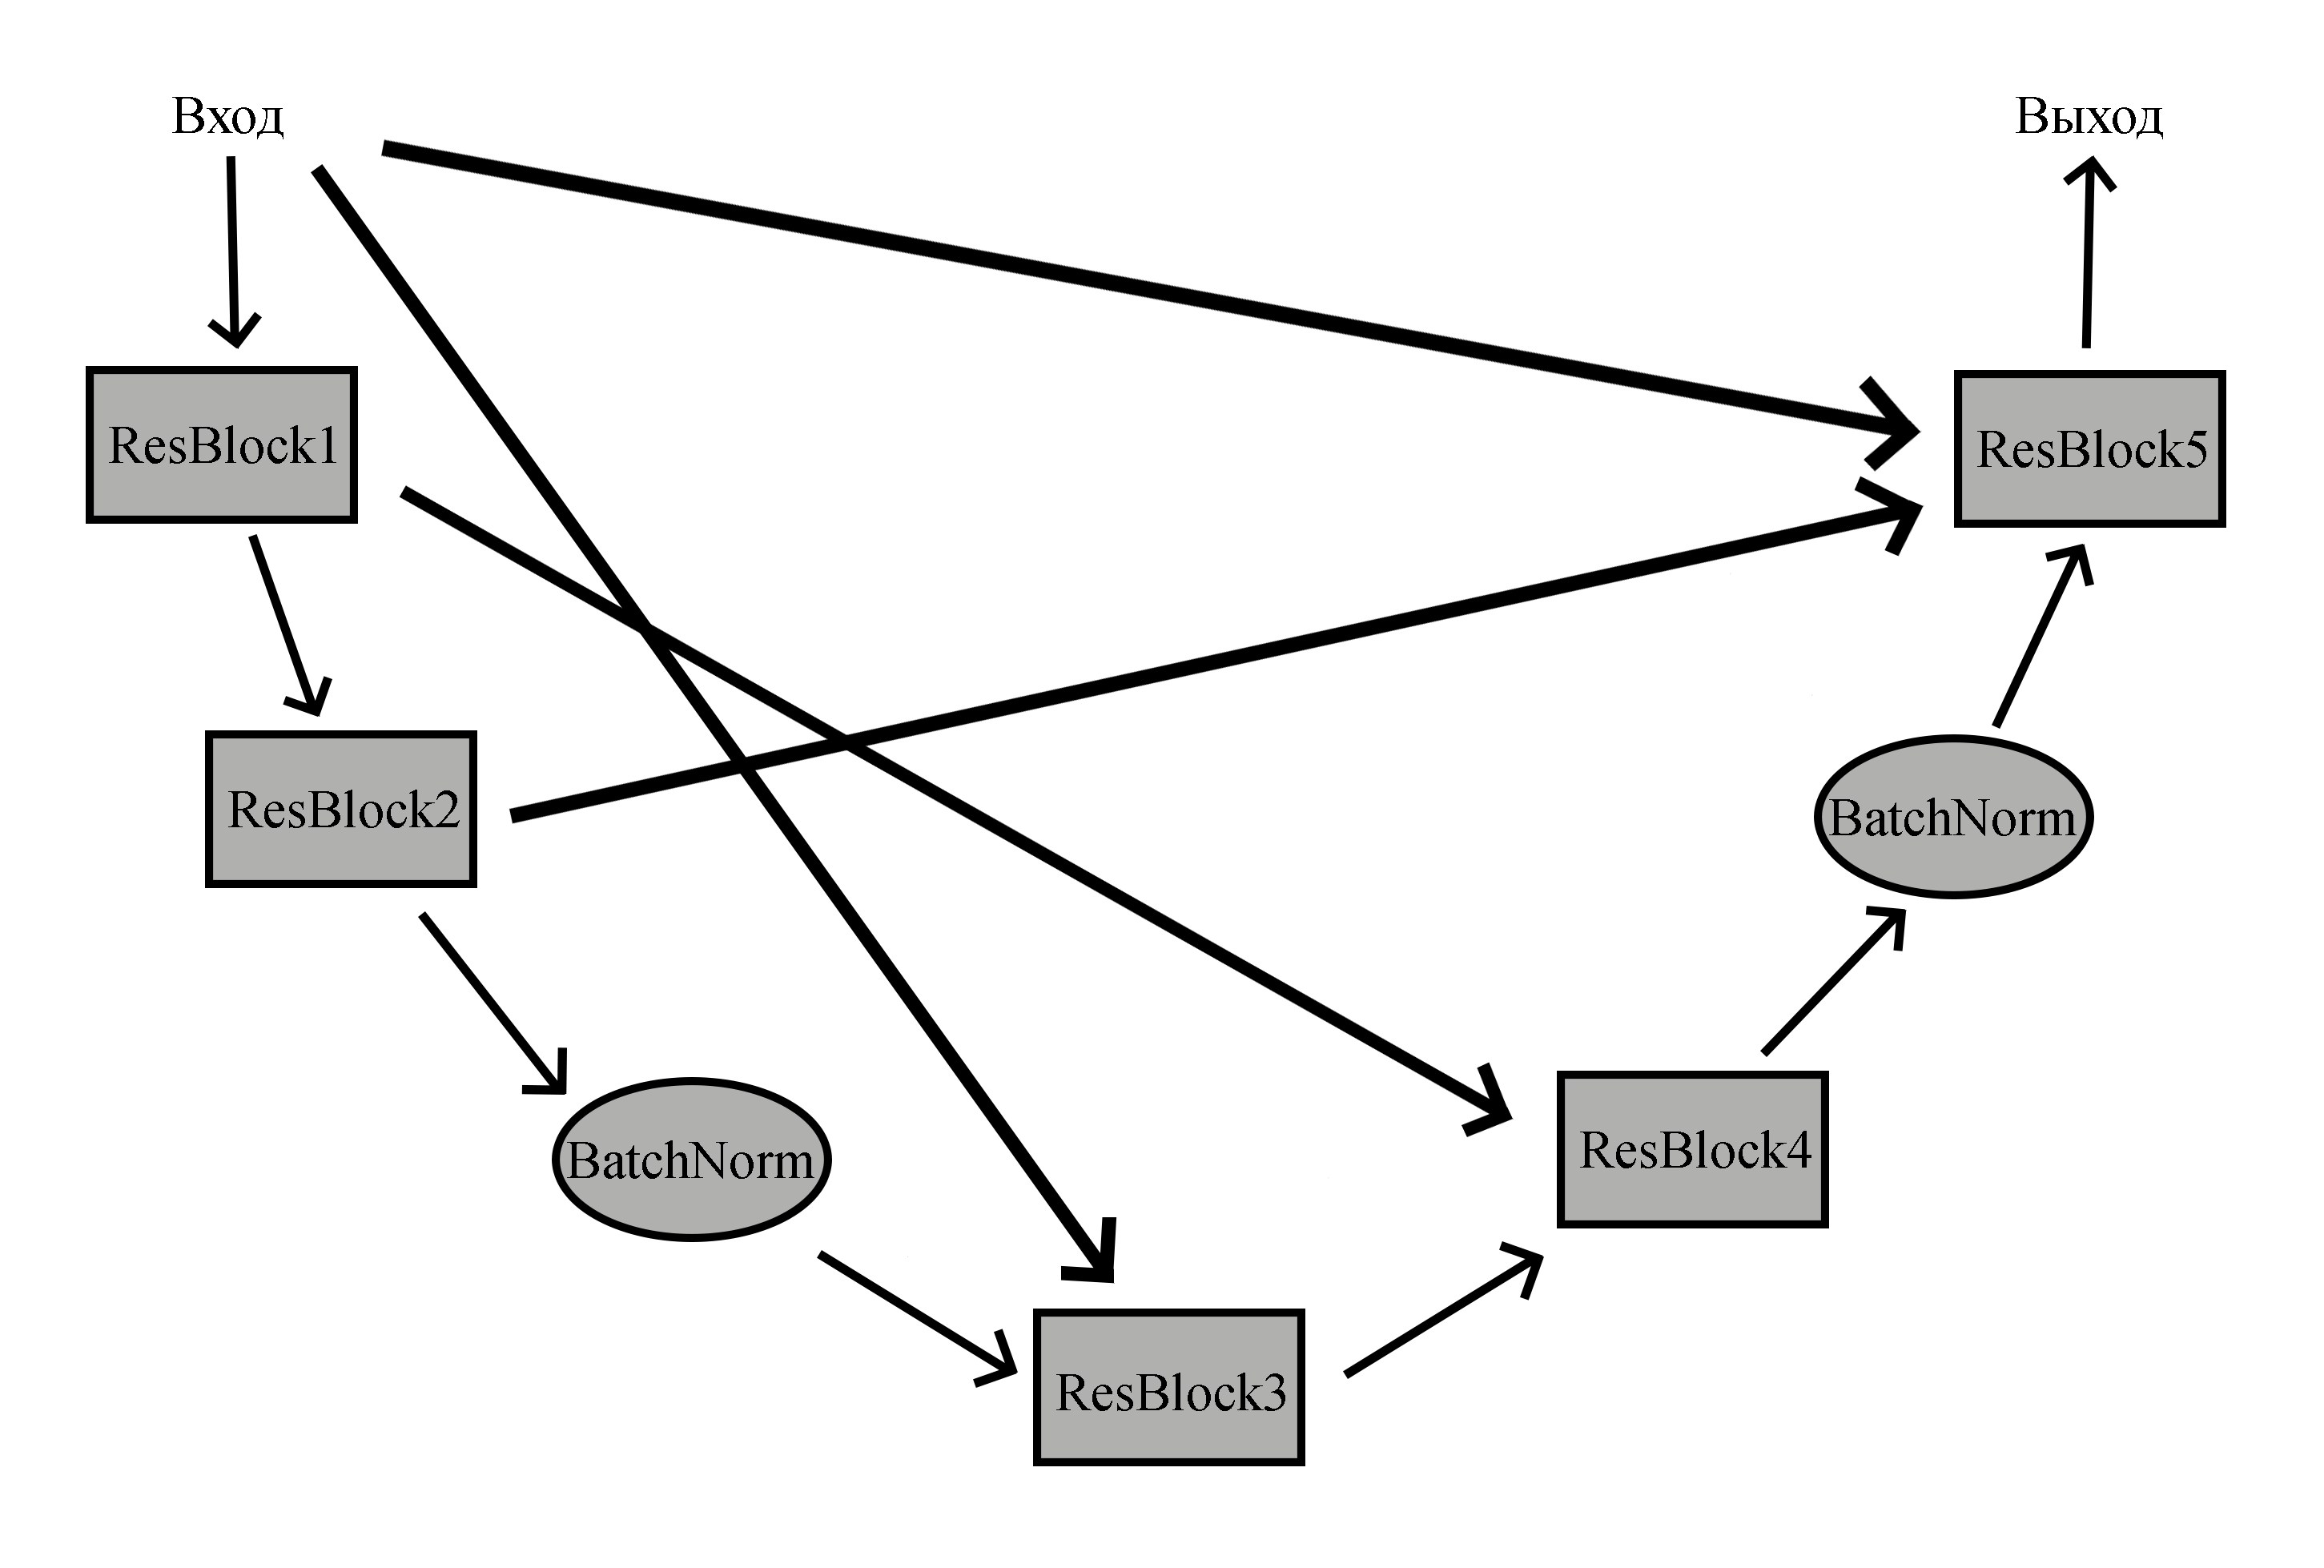
\includegraphics[width=\textwidth]{FCN5.png}
	\caption{Устройство сети FCN5.}
	\label{fig_fcn5}
\end{figure}

Сеть FCN5 по устройству крайне близка к сетям типа U-Net\cite{unet}, но сеть U-Net известна тем, что в ней количество каналов промежуточных тензоров сначала растёт, а потом убывает. При работе с FCN5, как и в большинстве других свёрточных сетей, количество каналов растёт всегда, за исключением, разве всего, последнего слоя.

Отметим, что количество каналов входного, а также количество выходных каналов в 5 остаточных слоях могут быть произвольными. В экспериментах часто использовалась следующая комбинация для промежуточных слоёв (входные каналы и пятый слой зависят от типа данных):
\begin{itemize}
\item Остаточный слой 1: 128 каналов;
\item Остаточный слой 2: 256 каналов;
\item Остаточный слой 3: 512 каналов;
\item Остаточный слой 4: 256, 384 или 512 каналов.
\end{itemize}
Для ускорения вычислений, также можно использовать уменьшенный вариант:
\begin{itemize}
\item Остаточный слой 1: 32 канала;
\item Остаточный слой 2: 64 канала;
\item Остаточный слой 3: 128 каналов;
\item Остаточный слой 4: 43 канала.
\end{itemize}

\subsection{Концепция сети-трансформера}
Основным недостатком полносвёрточных нейронных сетей является то, хоть они и могут обрабатывать изображения сколь угодно больших размеров (на сколько то позволяет память компьютера), для изображений крайне малого размера (которые в рамках данного исследования могут возникнуть при работе с пептидами), может оказаться, что применяемых свёрток слишком много (каждая свёртка уменьшает размер изображения, после чего операция паддинга возвращает исходный размер), и результат окажется совершенно ненадёжным. Также отметим, что операция свёртки локальна -- за формирования одного пикселя выходнного изображения отвечает ограниченная область вокруг этого пикселя в исходнном изображении. Это значит, что практически отстутствует связь между удалёнными участками изображения.

Наиболее привлекательным решением таких проблем выглядит использование сети-трансформера\cite{attention_all_you_need}. Такие сети в настоящее время получили крайне широкое распространение, прежде всего в задачах обработки естественного языка, но также и в задачах биоинформатики. Сети-трансформеры хорошо работают с данными, представленными в виде последовательностей, позволяют эффективно находить связи между удалёнными участками таких последовательностей.

Концептуально, в такой сети можно использовать токен, бинарно кодирующий 5 аминокислотных остатков и релятивистскую матрицу косинусов размера $4\times4$. На выходе можно, например, получать токены с матрицами косинусов $4\times4$, кодирующими матричное поле. Можно использовать и более простые выходные токены.

\section{Представление данных и процесс обучения нейронной сети}

\subsection{Набор данных}

Для создания набора данных использовались записи из банка данных PDB, опубликованные не позже 31 октября 2022. Была составлена программа, которая выявляла среди этих файлов модели белковых комплексов.
% 2-mer: 24370
% 3-mer: 4212
% 4-mer: 7987
% 5-mer: 732
% 6-mer: 2335
% 7-mer: 164
% 8-mer: 1270
% high-mer: 1853
С помощью неё было обнаружено:
\begin{itemize}
\item 24370 димерных комплексов;
\item 4212 тримерных комплексов;
\item 7987 4-мерных комплексов;
\item 732 5-мерных комплексов;
\item 2335 6-мерных комплексов;
\item 164 7-мерных комплексов;
\item 1270 8-мерных комплексов;
\item 1853 комплексов более высокого порядка.
\end{itemize}
% train: 19496
% valid: 4874

После фильтрации, которая включала в себя выделение всех попарных взаимодействий, исключая содержащие нестандартные аминоксилотные остатки, а также слишком короткие взаимодействующие молекулы, получили наборы данных из:
\begin{itemize}
\item 85014 взаимодействий в обучающем наборе; 
\item 21547 взаимодействий в тестовом наборе.
\end{itemize}
% train items: 85014
% valid items: 21547
% Oct 31 2022

\subsection{Процесс обучения}
Нейронная сеть обучается в течении нескольких больших итераций, называемых эпохами. Одна эпоха означает один полный обход обучающего набора данных, и валидацию на всём тестовом наборе. Каждую эпоху делят на некоторое число итераций, при которых выделяется фиксированный <<кусок>> обучающего набора данных (батч), который обрабатывается нейронной сетью. Результат оценивается с помощью некоторой функции потерь, после чего веса нейронной сети обновляются для минимизации этой самой функции потерь. Валидация тестового набора данных также производится по батчам.

В предлагаемом подходе, типичная итерация обучения выглядит следующим образом: 
\begin{enumerate}
\item Из набора данных выбирается следующий батч. Для этого в каждой записи о взаимодействии двух молекул выбирают пару взаимодействующих остатков, и производят обрезку обеих молекул под фиксированный размер так, чтобы взаимодействующая пара остатков сохранилась. Теперь, для сравнения, либо выбирают две рзличные точки, где взаимодействия нет (для \ref{L_multiscalar}), ложную модель взаимодействия. Координаты, закодированные аминокислотные остатки, а также координаты точек взаимодействия собирают в тензоры и отправляют на память видеокарты.
\item На видеокарте из координат атомов и точек взаимодействия строят соответствующую релятивистскую матрицу косинусов. Код аминокислотных остатков дополнительно обрабатывают и записывают в виде матрицы.
\item Нейросеть высчитывает матрицы косинусов, кодирующие обобщённые переменные поля для истинного и ложного взаимодействия. Переменные извлекаются из этих матриц, после чего считают частичные лагранжианы $L^{T}_{part}$ и $L^{F}_{part}$. 
\item В качестве функции потерь проще всего использовать разницу $L^{T}_{part} - L^{F}_{part}$, что будет приводить к тому, что истинным моделям будет сопоставляться меньший частичный лагранжиан, чем ложным. Но также желательно, чтобы выполнялось: $L^T_{part} < 0$ и $L^{F}_{part} > 0$. Поэтому использовалась следующая функция потерь:
\begin{equation}
	l(L^{T}_{part}, L^{F}_{part}) = \frac{(L^{T}_{part} - L^{F}_{part}) - \relu(-L^{T}_{part}) + \relu(-L^{F}_{part})}{2}.
	\label{loss_function}
\end{equation}
К данной функции также можно добавить значение (с маленьким весом), которое отражающую внутреннюю согласованность предсказанной матрицы косинусов (для этого из матрицы сначала получают обобщённые переменные, а потом по этим переменным опять строят матрицу, после чего считают разницу между первым и вторым).
\item Функция потерь $l(L^{T}_{part}, L^{F}_{part})$, посчитаная на текущем батче, минимизируется методом оптимизации Adam.
\end{enumerate}
\begin{figure}[H]
	\centering
	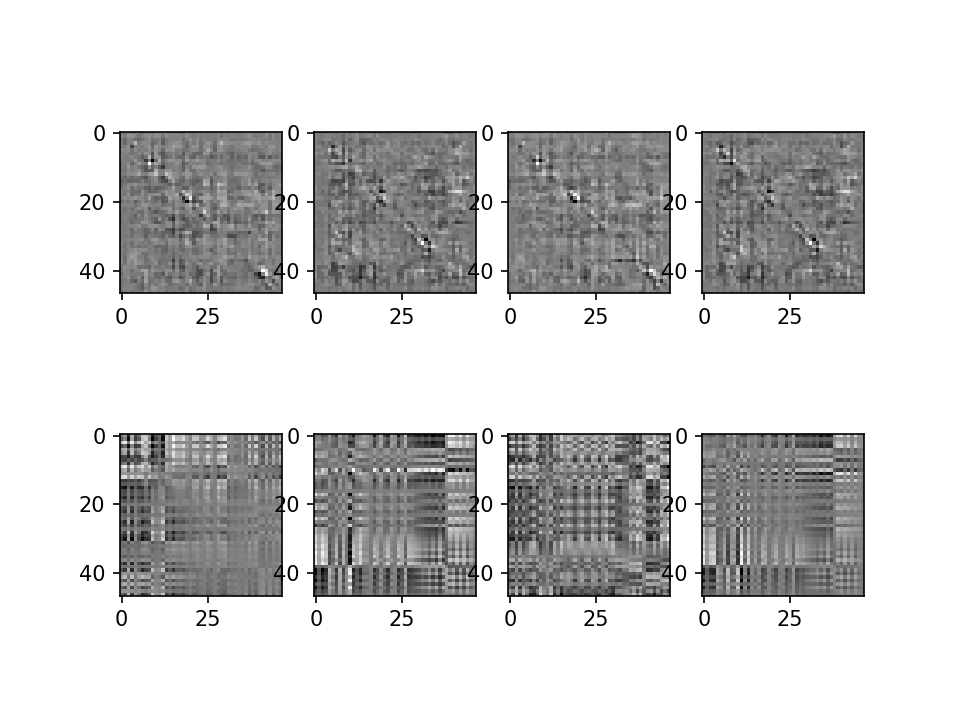
\includegraphics[width=\textwidth]{a5.png}
	\caption{Пример малой согласованности матриц. Верхняя строка -- выход нейронной сети, нижняя -- вид корректных матриц.}
	\label{fig_consistency}
\end{figure}


	\newpage
\begin{center}
	\textbf{\large ГЛАВА 6}

	\textbf{\large ВЫЧИСЛИТЕЛЬНЫЕ ЭКСПЕРИМЕНТЫ}
\end{center}
\refstepcounter{chapter}
\addcontentsline{toc}{chapter}{6. ВЫЧИСЛИТЕЛЬНЫЕ ЭКСПЕРИМЕНТЫ}

\section{Синтетические задачи}

\subsection{Задача №1}

\subsection{Задача №2}

\subsection{Задача №3}

\subsection{Задача №4}

\section{Моделирование полей для задачи взаимодействия белков}
	
	% Заключение
	\newpage
\begin{center}
	\textbf{\large ЗАКЛЮЧЕНИЕ}
\end{center}
\refstepcounter{chapter}
\addcontentsline{toc}{chapter}{ЗАКЛЮЧЕНИЕ}


Основные результаты магистерской квалификационной работы:
\begin{enumerate}
	
	\item Был продемонстрирован новый подход к описанию плавления в молекулярных системах, основанный на $\lambda^2$-параметре, который рассчитывается на основе разбиения системы частиц на ячейки Вороного.
	Показано, что разработанная модель демонстрирует существенно нелинейное поведение.
	Кроме того, предложенная модель позволяет с высокой степенью детализации изучать зародышеобразование в различных режимах перегрева и эволюцию жидких зародышей.
	
	\item Исследовано влияние формы потенциала парного взаимодействия на фазовые диаграммы и подвижность частиц в жидкой фазе.
	Рассчитаны кривые сосуществования газа и жидкости для потенциалов с переменной силой притяжения. 
	Установлено, что с увеличением дальнодействия потенциала температуры тройной и критической точек, а также их отношение $T_{\rm CP}/T_{\rm TP}$ увеличиваются. 
	Были рассчитаны коэффициент диффузии и коэффициент подвижности на жидких бинодалиях.
	Обнаружено, что температурная зависимость подвижности линейна в широком диапазоне температур с тем большим наклоном, чем меньше диапазон притяжения.
	Установлено, что начало нелинейной температурной зависимости подвижности при высоких температурах совпадает с переходом дисперсионных зависимостей коллективных возбуждений от осциллирующего к монотонному виду.
	
	\item Разработан новый метод распознавания фаз, основанный на алгоритме кластеризации DBSCAN.
	В совокупности с алгоритмом выделения поверхности метод позволяет с высокой точность рассчитывать фазовые диаграммы систем с различной плотностью и формами кластеров.
	Проведен сравнительный анализ различных методов построения фазовых диаграмм.
	Продемонстрировано, как новый метод распознавания фаз может быть применен к переохлажденным системам частиц для анализа скорости нуклеации при различном дальнодействии притяжения.
	
\end{enumerate}
	
	% Библиографический список
	\newpage
\addcontentsline{toc}{chapter}{СПИСОК ИСПОЛЬЗОВАННЫХ ИСТОЧНИКОВ} % это будет отображаться в содержании
\renewcommand{\bibsection}{\centering\textbf{\large СПИСОК ИСПОЛЬЗОВАННЫХ ИСТОЧНИКОВ}} % смена названия библиографии по умолчанию
%\bibliographystyle{biblio/gost2008n}
\bibliographystyle{plain}
%\bibliography{biblio/biblio}

\begin{thebibliography}{9}

\bibitem{prip2023}
Novikov, A. A. Prediction of protein-protein interaction with cosine matrices / A. A. Novikov, A. V. Tuzikov, A. V. Batyanovskii // Pattern Recognition and Information Processing (PRIP'2023) : Proceedings of the 16th International Conference, October 17–19, 2023, Minsk, Belarus / United Institute of Informatics Problems of the National Academy of Sciences of Belarus. – Minsk, 2023. – P. 258–263.

\bibitem{fully_conv}
Shelhamer, E. Fully convolutional networks for semantic segmentation / E. Shelhamer, J. Long // IEEE – 2015. – P. 1-12.

\bibitem{symmetry}
Exploring protein symmetry at the RCSB Protein Data Bank / J. Duarte [et al] // Emerging Topics in Life Sciences. – 2022. – P. 1-13.

\bibitem{vreven}
Vreven, T. Integrating atom-based and residue-based scoring functions for protein–protein docking / T.Vreven, H. Hwang, Z. Weng // Protein Sci. – 2011. – P. 1-11.

\bibitem{AF2}
Highly accurate protein structure prediction with AlphaFold / J. Jumper [et al] // Nature. – 2021. – P. 1-16.

\bibitem{AFM}
Protein complex prediction with AlphaFold-Multimer / R. Evans [et al] // DeepMind. – 2021. – P. 1-25.

\bibitem{AF3}
Accurate structure prediction of biomolecular interactions with AlphaFold 3 / J. Abramson [et al] // Nature. -- 2024. --P. 493-517.

\bibitem{AF_followers}
FastFold: Reducing AlphaFold Training Time from 11 Days to 67 Hours / S. Cheng [et al] // arXiv. – 2023. – P. 1-13.

\bibitem{andras}
Andras, S. Template-based structure modeling of protein-protein interactions / S. Andras, Y. Zhang // Curr Opin Struct Biol. – 2014. – P. 1-24.

\bibitem{deep_methods}
Deep Learning for Protein–Protein Interaction Site Prediction / R. Arian [et al.] // Methods Mol Biol. – 2021. – P. 1-26.

\bibitem{hang}
Hang, Y. Protein surface representation and analysis by dimension reduction / Y. Hang, R. Quershi, A. Sacan // Proteome Science. – 2012. – P. 1-13.

\bibitem{sverrisson}
Fast end-to-end learning on protein surfaces / F. Sverrisson [et al] // bioRxiv. – 2020. – P. 1-11.

\bibitem{guo}
Prediction of inter-chain distance maps of protein complexes with 2D attentionbased deep neural networks / Z. Guo [et al] // University of Missouri. – 2022. – P. 1-13.

\bibitem{hadarovich}
Хадарович, А. Ю. Алгоритмы моделирования димерных белковых комплексов / А. Ю. Хадарович // ОИПИ НАН. – 2020. – P. 1-100.

\bibitem{kufareva}
Kufareva, I. Methods of protein structure comparison / I. Kufareva, R. Abagyan // Methods Mol Biol. – 2012. – P. 1-30.

\bibitem{bradley}
Bradley, A. The use of the area under the ROC curve in the evaluation of machine learning algorithms / A. P. Bradley // Pattern Recognition. – 1997. – P. 1145-1159.

\bibitem{basu}
Basu, S. DockQ: A Quality Measure for Protein-Protein Docking Models / S. Basu, B. Wallner // PLoS ONE. – 2016. – P. 1-9.

\bibitem{zhu}
Evaluation of AlphaFold-Multimer prediction on multi-chain protein complexes / W. Zhu [et al] // Bioinformatics. -- 2023. -- P. 1-7.

\bibitem{field_theory}
Богуш, А.А. Введение в теорию классических полей / А. А. Богуш, Л. Г. Мороз. -- Изд. 2-е. -- М.: Едиториал УРСС, 2004. -- 384 с.

\bibitem{adam}
Kingma, D. Adam: A Method for Stochastic Optimization / D. Kingma, J. Ba // arXiv. -- 2017. -- P. 1-15.

\bibitem{evol_methods}
Eiben, A. Introduction to Evolutionary Computing / A.E. Eiben, J.E. Smith. -- 2nd ed. -- Berlin : Springer, 2015. -- XII, 287 p.

\bibitem{resnet}
Deep Residual Learning for Image Recognition / H. Kaiming [et al] // arXiv. – 2015. – P. 1-12.

\bibitem{batchnorm}
Ioffe, S. Batch Normalization: Accelerating Deep Network Training by Reducing Internal Covariate Shift / S. Ioffe, C. Szegedy // arXiv. – 2015. – P. 1-11.

\bibitem{unet}
Ronnenberger, O. U-Net: Convolutional Networks for Biomedical Image Segmentation / O. Ronnenberger, P. Fisher, T. Brox // arXiv. – 2015. – P. 1-8.

\bibitem{attention_all_you_need}
Attention Is All You Need / A. Vaswani [et al] // arXiv. – 2015. P. 1-15.

\end{thebibliography}
	
	% Приложение
	%\newpage
\begin{center}
	\textbf{\large ПРИЛОЖЕНИЕ А}
\end{center}
\refstepcounter{chapter}
\addcontentsline{toc}{chapter}{ПРИЛОЖЕНИЕ А}
	
\end{document}